\documentclass[]{book}
\usepackage{lmodern}
\usepackage{amssymb,amsmath}
\usepackage{ifxetex,ifluatex}
\usepackage{fixltx2e} % provides \textsubscript
\ifnum 0\ifxetex 1\fi\ifluatex 1\fi=0 % if pdftex
  \usepackage[T1]{fontenc}
  \usepackage[utf8]{inputenc}
\else % if luatex or xelatex
  \ifxetex
    \usepackage{mathspec}
  \else
    \usepackage{fontspec}
  \fi
  \defaultfontfeatures{Ligatures=TeX,Scale=MatchLowercase}
\fi
% use upquote if available, for straight quotes in verbatim environments
\IfFileExists{upquote.sty}{\usepackage{upquote}}{}
% use microtype if available
\IfFileExists{microtype.sty}{%
\usepackage{microtype}
\UseMicrotypeSet[protrusion]{basicmath} % disable protrusion for tt fonts
}{}
\usepackage[margin=1in]{geometry}
\usepackage{hyperref}
\hypersetup{unicode=true,
            pdftitle={Using R for Introduction to Econometrics},
            pdfauthor={Christoph Hanck, Martin Arnold, Alexander Gerber and Martin Schmelzer},
            pdfborder={0 0 0},
            breaklinks=true}
\urlstyle{same}  % don't use monospace font for urls
\usepackage{natbib}
\bibliographystyle{apa}
\usepackage{color}
\usepackage{fancyvrb}
\newcommand{\VerbBar}{|}
\newcommand{\VERB}{\Verb[commandchars=\\\{\}]}
\DefineVerbatimEnvironment{Highlighting}{Verbatim}{commandchars=\\\{\}}
% Add ',fontsize=\small' for more characters per line
\usepackage{framed}
\definecolor{shadecolor}{RGB}{248,248,248}
\newenvironment{Shaded}{\begin{snugshade}}{\end{snugshade}}
\newcommand{\KeywordTok}[1]{\textcolor[rgb]{0.13,0.29,0.53}{\textbf{#1}}}
\newcommand{\DataTypeTok}[1]{\textcolor[rgb]{0.13,0.29,0.53}{#1}}
\newcommand{\DecValTok}[1]{\textcolor[rgb]{0.00,0.00,0.81}{#1}}
\newcommand{\BaseNTok}[1]{\textcolor[rgb]{0.00,0.00,0.81}{#1}}
\newcommand{\FloatTok}[1]{\textcolor[rgb]{0.00,0.00,0.81}{#1}}
\newcommand{\ConstantTok}[1]{\textcolor[rgb]{0.00,0.00,0.00}{#1}}
\newcommand{\CharTok}[1]{\textcolor[rgb]{0.31,0.60,0.02}{#1}}
\newcommand{\SpecialCharTok}[1]{\textcolor[rgb]{0.00,0.00,0.00}{#1}}
\newcommand{\StringTok}[1]{\textcolor[rgb]{0.31,0.60,0.02}{#1}}
\newcommand{\VerbatimStringTok}[1]{\textcolor[rgb]{0.31,0.60,0.02}{#1}}
\newcommand{\SpecialStringTok}[1]{\textcolor[rgb]{0.31,0.60,0.02}{#1}}
\newcommand{\ImportTok}[1]{#1}
\newcommand{\CommentTok}[1]{\textcolor[rgb]{0.56,0.35,0.01}{\textit{#1}}}
\newcommand{\DocumentationTok}[1]{\textcolor[rgb]{0.56,0.35,0.01}{\textbf{\textit{#1}}}}
\newcommand{\AnnotationTok}[1]{\textcolor[rgb]{0.56,0.35,0.01}{\textbf{\textit{#1}}}}
\newcommand{\CommentVarTok}[1]{\textcolor[rgb]{0.56,0.35,0.01}{\textbf{\textit{#1}}}}
\newcommand{\OtherTok}[1]{\textcolor[rgb]{0.56,0.35,0.01}{#1}}
\newcommand{\FunctionTok}[1]{\textcolor[rgb]{0.00,0.00,0.00}{#1}}
\newcommand{\VariableTok}[1]{\textcolor[rgb]{0.00,0.00,0.00}{#1}}
\newcommand{\ControlFlowTok}[1]{\textcolor[rgb]{0.13,0.29,0.53}{\textbf{#1}}}
\newcommand{\OperatorTok}[1]{\textcolor[rgb]{0.81,0.36,0.00}{\textbf{#1}}}
\newcommand{\BuiltInTok}[1]{#1}
\newcommand{\ExtensionTok}[1]{#1}
\newcommand{\PreprocessorTok}[1]{\textcolor[rgb]{0.56,0.35,0.01}{\textit{#1}}}
\newcommand{\AttributeTok}[1]{\textcolor[rgb]{0.77,0.63,0.00}{#1}}
\newcommand{\RegionMarkerTok}[1]{#1}
\newcommand{\InformationTok}[1]{\textcolor[rgb]{0.56,0.35,0.01}{\textbf{\textit{#1}}}}
\newcommand{\WarningTok}[1]{\textcolor[rgb]{0.56,0.35,0.01}{\textbf{\textit{#1}}}}
\newcommand{\AlertTok}[1]{\textcolor[rgb]{0.94,0.16,0.16}{#1}}
\newcommand{\ErrorTok}[1]{\textcolor[rgb]{0.64,0.00,0.00}{\textbf{#1}}}
\newcommand{\NormalTok}[1]{#1}
\usepackage{longtable,booktabs}
\usepackage{graphicx,grffile}
\makeatletter
\def\maxwidth{\ifdim\Gin@nat@width>\linewidth\linewidth\else\Gin@nat@width\fi}
\def\maxheight{\ifdim\Gin@nat@height>\textheight\textheight\else\Gin@nat@height\fi}
\makeatother
% Scale images if necessary, so that they will not overflow the page
% margins by default, and it is still possible to overwrite the defaults
% using explicit options in \includegraphics[width, height, ...]{}
\setkeys{Gin}{width=\maxwidth,height=\maxheight,keepaspectratio}
\IfFileExists{parskip.sty}{%
\usepackage{parskip}
}{% else
\setlength{\parindent}{0pt}
\setlength{\parskip}{6pt plus 2pt minus 1pt}
}
\setlength{\emergencystretch}{3em}  % prevent overfull lines
\providecommand{\tightlist}{%
  \setlength{\itemsep}{0pt}\setlength{\parskip}{0pt}}
\setcounter{secnumdepth}{5}
% Redefines (sub)paragraphs to behave more like sections
\ifx\paragraph\undefined\else
\let\oldparagraph\paragraph
\renewcommand{\paragraph}[1]{\oldparagraph{#1}\mbox{}}
\fi
\ifx\subparagraph\undefined\else
\let\oldsubparagraph\subparagraph
\renewcommand{\subparagraph}[1]{\oldsubparagraph{#1}\mbox{}}
\fi

%%% Use protect on footnotes to avoid problems with footnotes in titles
\let\rmarkdownfootnote\footnote%
\def\footnote{\protect\rmarkdownfootnote}

%%% Change title format to be more compact
\usepackage{titling}

% Create subtitle command for use in maketitle
\newcommand{\subtitle}[1]{
  \posttitle{
    \begin{center}\large#1\end{center}
    }
}

\setlength{\droptitle}{-2em}

  \title{Using R for Introduction to Econometrics}
    \pretitle{\vspace{\droptitle}\centering\huge}
  \posttitle{\par}
    \author{Christoph Hanck, Martin Arnold, Alexander Gerber and Martin Schmelzer}
    \preauthor{\centering\large\emph}
  \postauthor{\par}
      \predate{\centering\large\emph}
  \postdate{\par}
    \date{2018-07-17}

\usepackage{booktabs}
%\usepackage{amsmath}
\usepackage{amsthm}
\usepackage{float}
\usepackage{rotating, graphicx}
\usepackage{multirow}
\usepackage{tabularx}

\newcommand{\comma}{,\,}

\floatplacement{figure}{H}

\PassOptionsToPackage{table}{xcolor}

\usepackage{tcolorbox}

\definecolor{kcblue}{HTML}{D7DDEF}
\definecolor{kcdarkblue}{HTML}{2B4E70}

\makeatletter
\def\thm@space@setup{%
  \thm@preskip=8pt plus 2pt minus 4pt
  \thm@postskip=\thm@preskip
}
\makeatother

\makeatletter % undo the wrong changes made by mathspec
\let\RequirePackage\original@RequirePackage
\let\usepackage\RequirePackage
\makeatother

\newenvironment{rmdknit}
    {\begin{center}
    \begin{tabular}{|p{0.9\textwidth}|}
    \hline\\
    }
    {
    \\\\\hline
    \end{tabular}
    \end{center}
    }

\newenvironment{rmdnote}
    {\begin{center}
    \begin{tabular}{|p{0.9\textwidth}|}
    \hline\\
    }
    {
    \\\\\hline
    \end{tabular}
    \end{center}
    }

\newtcolorbox[auto counter, number within=section]{keyconcepts}[2][]{%
colback=kcblue,colframe=kcdarkblue,fonttitle=\bfseries, title=Key Concept~#2, after title={\newline #1}, beforeafter skip=15pt}

\usepackage{amsthm}
\newtheorem{theorem}{Theorem}[chapter]
\newtheorem{lemma}{Lemma}[chapter]
\theoremstyle{definition}
\newtheorem{definition}{Definition}[chapter]
\newtheorem{corollary}{Corollary}[chapter]
\newtheorem{proposition}{Proposition}[chapter]
\theoremstyle{definition}
\newtheorem{example}{Example}[chapter]
\theoremstyle{definition}
\newtheorem{exercise}{Exercise}[chapter]
\theoremstyle{remark}
\newtheorem*{remark}{Remark}
\newtheorem*{solution}{Solution}
\begin{document}
\maketitle

{
\setcounter{tocdepth}{1}
\tableofcontents
}
\chapter{Introduction}\label{introduction}

\begin{center}
\includegraphics[width=0.45\linewidth]{images/URFITE_logo} \end{center}

\noindent\rule{\textwidth}{1pt}

The interest in the freely available statistical programming language
and software environment \texttt{R} is soaring. By the time we wrote
first drafts for this project, more than 11000 addons (many of them
providing cutting-edge methods) were made available on the Comprehensive
\texttt{R} Archive Network (\href{https://cran.r-project.org/}{CRAN}),
an extensive network of FTP servers around the world that store
identical and up-to-date versions of \texttt{R} code and its
documentation. \texttt{R} dominates other (commercial) software for
statistical computing in most fields of research in applied statistics.
The benefits of it being freely available, open source and having a
large and constantly growing community of users that contribute to CRAN
render \texttt{R} more and more appealing for empirical economists and
econometricians as well.

A striking advantage of using \texttt{R} in econometrics courses is that
it enables students to explicitly document their analysis step-by-step
such that it is easy to update and to expand. This allows to re-use code
for similar applications with different data. Furthermore, \texttt{R}
programs are fully reproducible which makes it straightforward for
others to comprehend and validate results.

Over the recent years, \texttt{R} has thus become an integral part of
the curricula of econometrics classes we teach at University of
Duisburg-Essen. In some sense, learning to code is comparable to
learning a foreign language and continuous practice is essential for the
learning success. Of course, presenting bare \texttt{R} code chunks on
slides has mostly a deterring effect for the students to engage with
programming on their own. This is why we offer tutorials where both
econometric theory and its applications using \texttt{R} are introduced,
for some time now. As for accompanying literature, there are some
excellent books that deal with \texttt{R} and its applications to
econometrics like \citet{kleiber2008}. However, we have found that these
works are somewhat difficult to access, especially for undergraduate
students in economics having little understanding of econometric methods
and predominantly no experience in programming at all. Consequently, we
have started to compile a collection of reproducible reports for use in
class. These reports provide guidance on how to implement selected
applications from the textbook \emph{Introduction to Econometrics}
\citep{stock2015} which serves as a basis for the lecture and the
accompanying tutorials. The process has been facilitated considerably
with the release of \texttt{knitr} (2018). \texttt{knitr} is an
\texttt{R} package for dynamic report generation which allows to
seamlessly combine pure text, LaTeX, \texttt{R} code and its output in a
variety of formats, including PDF and HTML. Being inspired by
\emph{Using R for Introductory Econometrics} \citep{heiss2016}\footnote{\citet{heiss2016}
  builds on the popular \emph{Introductory Econometrics} by
  \citet{wooldridge2016} and demonstrates how to replicate the
  applications discussed therein using \texttt{R}.} and with this
powerful toolkit at hand we decided to write up our own empirical
companion to \citet{stock2015} which resulted in \textbf{U}sing
\textbf{R} \textbf{f}or \textbf{I}ntroduction \textbf{t}o
\textbf{E}conometrics (\emph{URFITE}).

Similarly to the book by \citet{heiss2016} this project is neither a
comprehensive econometrics textbook nor is it intended to be a general
introduction \texttt{R}. \emph{URFITE} is best described as an
interactive script in the style of a reproducible research report which
aims to provide students of economic sciences with a
platform-independent e-learning arrangement by seamlessly intertwining
theoretical core knowledge and empirical skills in undergraduate
econometrics. Of course the focus is set on empirical applications with
\texttt{R}; we leave out tedious derivations and formal proofs wherever
we can. \emph{URFITE} is closely aligned on \citet{stock2015} which does
very well in motivating theory by real-world applications. However, we
take it a step further and enable students not only to learn how results
of case studies can be replicated with \texttt{R} but we also intend to
strengthen their ability in using the newly acquired skills in other
empirical applications. To support this, each chapter contains
interactive \texttt{R} programming exercises. These exercises are used
as supplements to code chunks that display how previously discussed
techniques can be implemented within \texttt{R}. They are generated
using the \href{https://github.com/datacamp/datacamp-light}{DataCamp
light widget} and are backed by an \texttt{R}-session which is
maintained on \href{https://www.datacamp.com/home}{DataCamp}'s servers.
You may play around with the example exercise presented below.

\begin{center}\textit{This interactive application is only available in the HTML version.}\end{center}

As you can see above, the widget consists of two tabs. \texttt{script.R}
mimics an \texttt{.R}-file, a file format that is commonly used for
storing \texttt{R} code. Lines starting with a \# are commented out,
that is they are not recognized as code. Furthermore, \texttt{script.R}
works like an exercise sheet where you may write down the solution you
come up with. If you hit the button \emph{Run}, the code will be
executed, submission correctness tests are run and you will be notified
whether your approach is correct. If it is not correct, you will receive
feedback suggesting improvements or hints. The other tab,
\texttt{R Console}, is a fully functional \texttt{R} console that can be
used for trying out solutions to exercises before submitting them. Of
course you may submit (almost any) arbitrary \texttt{R} code and use the
console to play around and explore. Simply type a command and hit the
enter key on your keyboard.

As an example, consider the following line of code presented in chunk
below. It tells \texttt{R} to compute the number of packages available
on \texttt{CRAN}. The code chunk is followed by the output produced.

\begin{Shaded}
\begin{Highlighting}[]
\CommentTok{# compute the number of packages available on CRAN}
\KeywordTok{nrow}\NormalTok{(}\KeywordTok{available.packages}\NormalTok{(}\DataTypeTok{repos =} \StringTok{"http://cran.us.r-project.org"}\NormalTok{))}
\end{Highlighting}
\end{Shaded}

\begin{verbatim}
## [1] 12740
\end{verbatim}

Each code chunk is equipped with a button on the outer right hand side
which copies the code to your clipboard. This makes it convenient to
work with larger code segments. In the widget above, you may click on
\texttt{R Console} and type \texttt{nrow(available.packages())} (the
command from the code chunk above) and execute it by hitting
\emph{Enter} on your keyboard\footnote{The \texttt{R} session is
  initialized by clicking anywhere into the widget. This might take a
  few seconds. Just wait for the indicator next to the button \emph{Run}
  to turn green}.

As you might have noticed, there are some out-commented lines in the
widget that ask you to assign a numeric value to a variable and then to
print the variable's content to the console. You may enter your solution
approach to \texttt{script.R} and hit the button \emph{Run} in order to
get the feedback described further above. In case you do not know how to
solve this sample exercise (don't panic, that is probably why you are
reading this), a click on \emph{Hint} will prompt you with some advice.
If you still can't find a solution, a click on \emph{solution} will
provide you with another tab, \texttt{Solution.R} which contains sample
solution code. It will often be the case that exercises can be solved in
many different ways and \texttt{Solution.R} presents what we consider as
comprehensible and idiomatic.

\subsubsection*{Conventions Used in this
Book}\label{conventions-used-in-this-book}
\addcontentsline{toc}{subsubsection}{Conventions Used in this Book}

\begin{itemize}
\item
  \emph{Italic} text indicates new terms, names, buttons and alike.
\item
  \texttt{Constant width text}, is generally used in paragraphs to refer
  to \texttt{R} code. This includes commands, variables, functions, data
  types, databases and file names.
\item
  Constant width text on gray background is used to indicate \texttt{R}
  code that can be typed literally by you. It may appear in paragraphs
  for better distinguishability among executable and non-executable code
  statements but it will mostly be encountered in shape of large blocks
  of \texttt{R} code. These blocks are referred to as code chunks (see
  above).
\end{itemize}

\subsubsection*{Acknowledgements}\label{acknowledgements}
\addcontentsline{toc}{subsubsection}{Acknowledgements}

We thank Alexander Blasberg and Kim Hermann for proofreading and their
constructive criticism.

\section{\texorpdfstring{A Very Short Introduction to \texttt{R} and
\emph{RStudio}}{A Very Short Introduction to  and RStudio}}\label{a-very-short-introduction-to-and-rstudio}

\begin{figure}[h]

{\centering 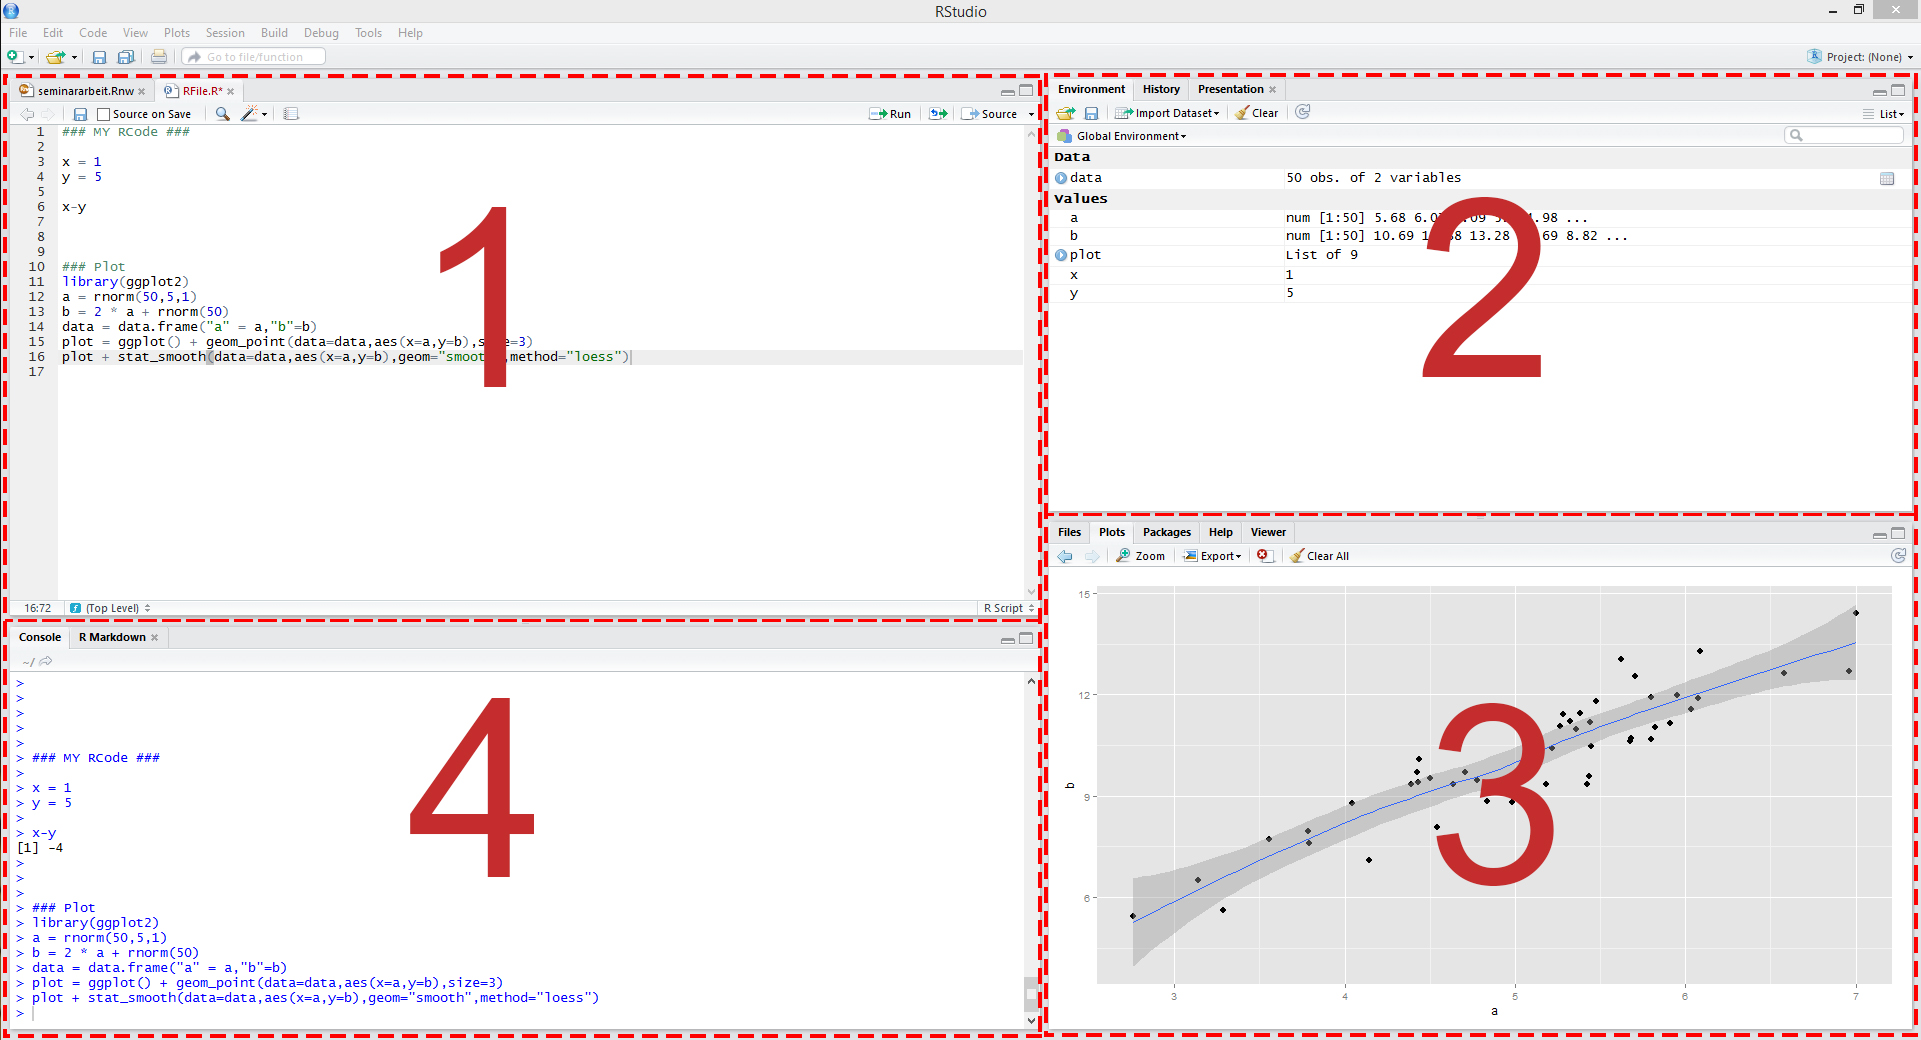
\includegraphics[width=1\linewidth]{images/rstudio} 

}

\caption{RStudio: the four panes}\label{fig:unnamed-chunk-7}
\end{figure}

\subsubsection*{\texorpdfstring{\texttt{R}
Basics}{ Basics}}\label{basics}
\addcontentsline{toc}{subsubsection}{\texttt{R} Basics}

This section is meant for those who have never worked with \texttt{R} or
\emph{RStudio}. If you at least know how to create objects and call
functions, you can skip it. If you would like to refresh your memories
or get a feeling for how to work with \emph{RStudio}, keep reading.

First of all start \emph{RStudio} and create a new R Script by selecting
\emph{File}, \emph{New File}, \emph{R Script}. In the editor pane type

\begin{Shaded}
\begin{Highlighting}[]
\DecValTok{1} \OperatorTok{+}\StringTok{ }\DecValTok{1}
\end{Highlighting}
\end{Shaded}

and click on the button labeled \emph{Run} in the top right corner of
the editor. By doing so, your line of code is send to the console and
the result of this operation should be displayed right underneath it. As
you can see, \texttt{R} works just like a calculator. You can do all the
arithmetic calculations by using the corresponding operator (+, - , *, /
or \^{}). If you are not sure what the last operator does, try it out
and check the results.

\subsubsection*{Vectors}\label{vectors}
\addcontentsline{toc}{subsubsection}{Vectors}

\texttt{R} is of course more sophisticated than that. We can work with
variables or more generally objects. Objects are defined by using the
assignment operator \texttt{<-}. To create a variable named \texttt{x}
which contains the value \texttt{10} type \texttt{x\ \textless{}-\ 10}
and click the button \emph{Run} yet again. The new variable should have
appeared in the environment pane on the top right. The console however
did not show any results, because our line of code did not contain any
call that creates output. When you now type \texttt{x} in the console
and hit return, you ask \texttt{R} to show you the value of \texttt{x}
and the corresponding value should be printed in the console.

\texttt{x} is a scalar, a vector of length \(1\). You can easily create
longer vectors by using the function \texttt{c()} (\emph{c} for
``concatenate'' or ``combine''). To create a vector \texttt{y}
containing the numbers \(1\) to \(5\) and print it, do the following.

\begin{Shaded}
\begin{Highlighting}[]
\NormalTok{y <-}\StringTok{ }\KeywordTok{c}\NormalTok{(}\DecValTok{1}\NormalTok{, }\DecValTok{2}\NormalTok{, }\DecValTok{3}\NormalTok{, }\DecValTok{4}\NormalTok{, }\DecValTok{5}\NormalTok{)}
\NormalTok{y}
\end{Highlighting}
\end{Shaded}

\begin{verbatim}
## [1] 1 2 3 4 5
\end{verbatim}

You can also create a vector of letters or words. For now just remember
that characters have to be surrounded by quotes, else wise they will be
parsed as object names.

\begin{Shaded}
\begin{Highlighting}[]
\NormalTok{hello <-}\StringTok{ }\KeywordTok{c}\NormalTok{(}\StringTok{"Hello"}\NormalTok{, }\StringTok{"World"}\NormalTok{)}
\end{Highlighting}
\end{Shaded}

Here we have created a vector of length 2 containing the words
\texttt{Hello} and \texttt{World}.

Do not forget to save your script! To do so, select \emph{File},
\emph{Save}.

\subsubsection*{Functions}\label{functions}
\addcontentsline{toc}{subsubsection}{Functions}

You have seen the function \texttt{c()} that can be used to combine
objects. In general, function calls look all the same, a function name
is always followed by round parentheses. Sometimes, the parentheses
include arguments

Here are two simple examples.

\begin{Shaded}
\begin{Highlighting}[]
\NormalTok{z <-}\StringTok{ }\KeywordTok{seq}\NormalTok{(}\DataTypeTok{from =} \DecValTok{1}\NormalTok{, }\DataTypeTok{to =} \DecValTok{5}\NormalTok{, }\DataTypeTok{by =} \DecValTok{1}\NormalTok{)}

\KeywordTok{mean}\NormalTok{(}\DataTypeTok{x =}\NormalTok{ z)}
\end{Highlighting}
\end{Shaded}

\begin{verbatim}
## [1] 3
\end{verbatim}

In the first line we use a function called \texttt{seq} to create the
exact same vector as we did in the previous section but naming it
\texttt{z}. The function takes on the arguments \texttt{from},
\texttt{to} and \texttt{by} which should be self-explaining. The
function \texttt{mean()} computes the arithmetic mean of its argument
\texttt{x}. Since we pass the vector \texttt{z} as the argument
\texttt{x} to \texttt{mean()}, the result is \texttt{3}!

If you are not sure what argument a function expects you may consult the
function's documentation. Let's say we are not sure how the arguments
required for \texttt{seq()} work. Then we can type \texttt{?seq} in the
console and by hitting return the documentation page for that function
pops up in the lower right pane of \emph{RStudio}. In there, the section
\emph{Arguments} holds the information we seek.

On the bottom of almost every help page you find examples on how to use
the corresponding functions. This is very helpful for beginners and we
recommend to look out for those.

\chapter{Regression with a Binary Dependent Variable}\label{rwabdv}

In this chapter, we discuss a special class of regression models that
aims to explain a limited dependent variable by multiple regressors.

In particular, we consider models where the dependent variable is
binary. We will see that in such models, the regression function can be
interpreted as a conditional probability function of the binary
dependent variable.

We review the following concepts:

\begin{itemize}
\tightlist
\item
  The linear probability model
\item
  The Probit model
\item
  The Logit model
\item
  Maximum likelihood estimation of nonlinear regression models
\end{itemize}

Of course, we will also see how to estimate abovementioned models using
\texttt{R} and discuss an application where we examine the question
whether there is racial discrimination in the U.S. mortgage market.

The following packages and their dependencies are needed for
reproduction of the code chunks presented throughout this chapter on
your computer:

\begin{itemize}
\tightlist
\item
  \texttt{AER}
\item
  \texttt{stargazer}
\end{itemize}

Check whether the following code chunk runs without any errors.

\begin{Shaded}
\begin{Highlighting}[]
\KeywordTok{library}\NormalTok{(AER)}
\KeywordTok{library}\NormalTok{(stargazer)}
\end{Highlighting}
\end{Shaded}

\section{Binary Dependent Variables and the Linear Probability
Model}\label{binary-dependent-variables-and-the-linear-probability-model}

\begin{keyconcepts}[The Linear Probability Model]{11.1}
The linear regression model 
$$Y_i = \beta_0 + \beta_1 + X_{1i} + \beta_2 X_{2i} + \dots + \beta_k X_{ki} + u_i$$
with a binary dependent variable $Y_i$ is called the linear probability model. In the linear probability model we have $$E(Y\vert X_1,X_2,\dots,X_k) = P(Y=1\vert X_1, X_2,\dots, X_3)$$ such that $$ P(Y = 1 \vert X_1, X_2, \dots, X_k) = \beta_0 + \beta_1 + X_{1i} + \beta_2 X_{2i} + \dots + \beta_k X_{ki}.$$\newline

Thus, the coefficient $\beta_j$ can be interpreted as the change in the probability that $Y_i=1$, holding constant the other $k-1$ regressors. Just as in common multiple regression, the $\beta_j$ can be estimated using OLS and the robust standard error formulas can be used for hypothesis testing and computation of confidence intervals.\newline 

In most linear probability models, $R^2$ has no meaningful interpretation since the regression line can never fit the data perfectly if the dependent variable is binary and the regressors are continuous. This can be seen in the application below.\newline

We emphasize that it is \textit{essential} to use robust standard errors since the $u_i$ in a linear probability model are always heteroskedastic.\newline

Linear probability models are easily estimated in \texttt{R} using the function exttt{lm()}.
\end{keyconcepts}

\subsubsection*{Mortgage Data}\label{mortgage-data}
\addcontentsline{toc}{subsubsection}{Mortgage Data}

Following the book, we start by loading the data set \texttt{HMDA} which
provides data that relate to mortgage applications filed in Boston in
the year of 1990.

\begin{Shaded}
\begin{Highlighting}[]
\CommentTok{# load `AER` package and attach the HMDA data}
\KeywordTok{library}\NormalTok{(AER)}
\KeywordTok{data}\NormalTok{(HMDA)}
\end{Highlighting}
\end{Shaded}

We continue by inspecting the first few observations and compute summary
statistics afterwards.

\begin{Shaded}
\begin{Highlighting}[]
\CommentTok{# Inspect data}
\KeywordTok{head}\NormalTok{(HMDA)}
\end{Highlighting}
\end{Shaded}

\begin{verbatim}
##   deny pirat hirat     lvrat chist mhist phist unemp selfemp insurance
## 1   no 0.221 0.221 0.8000000     5     2    no   3.9      no        no
## 2   no 0.265 0.265 0.9218750     2     2    no   3.2      no        no
## 3   no 0.372 0.248 0.9203980     1     2    no   3.2      no        no
## 4   no 0.320 0.250 0.8604651     1     2    no   4.3      no        no
## 5   no 0.360 0.350 0.6000000     1     1    no   3.2      no        no
## 6   no 0.240 0.170 0.5105263     1     1    no   3.9      no        no
##   condomin afam single hschool
## 1       no   no     no     yes
## 2       no   no    yes     yes
## 3       no   no     no     yes
## 4       no   no     no     yes
## 5       no   no     no     yes
## 6       no   no     no     yes
\end{verbatim}

\begin{Shaded}
\begin{Highlighting}[]
\KeywordTok{summary}\NormalTok{(HMDA)}
\end{Highlighting}
\end{Shaded}

\begin{verbatim}
##   deny          pirat            hirat            lvrat        chist   
##  no :2095   Min.   :0.0000   Min.   :0.0000   Min.   :0.0200   1:1353  
##  yes: 285   1st Qu.:0.2800   1st Qu.:0.2140   1st Qu.:0.6527   2: 441  
##             Median :0.3300   Median :0.2600   Median :0.7795   3: 126  
##             Mean   :0.3308   Mean   :0.2553   Mean   :0.7378   4:  77  
##             3rd Qu.:0.3700   3rd Qu.:0.2988   3rd Qu.:0.8685   5: 182  
##             Max.   :3.0000   Max.   :3.0000   Max.   :1.9500   6: 201  
##  mhist    phist          unemp        selfemp    insurance  condomin  
##  1: 747   no :2205   Min.   : 1.800   no :2103   no :2332   no :1694  
##  2:1571   yes: 175   1st Qu.: 3.100   yes: 277   yes:  48   yes: 686  
##  3:  41              Median : 3.200                                   
##  4:  21              Mean   : 3.774                                   
##                      3rd Qu.: 3.900                                   
##                      Max.   :10.600                                   
##   afam      single     hschool   
##  no :2041   no :1444   no :  39  
##  yes: 339   yes: 936   yes:2341  
##                                  
##                                  
##                                  
## 
\end{verbatim}

The variable we are interested in modelling is \texttt{deny}, an
indicator for whether an applicants mortgage application has been
accepted (\texttt{deny = no}) or denied (\texttt{deny = yes}). A
regressors that can be presumed to have power in explaining whether a
mortgage application has been denied or accepted is \texttt{pirat}, the
size of the anticipated total monthly loan payments relative to the the
applicant's income. It is straightforward to translate this into the
simple regression model

\begin{align}
  deny = \beta_0 + \beta_1 P/I\ ratio + u. \label{eq:denymod1}
\end{align}

We can estimate this model just as any other linear regression model
using \texttt{lm()}. Before we do so, the variable \texttt{deny} must be
converted to a numeric variable using \texttt{as.numeric()}. Note that
\texttt{as.numeric(HMDA\textbackslash{}\$deny)} will turn
\texttt{deny = no} into \texttt{deny = 1} and \texttt{deny = yes} into
\texttt{deny = 2}, so using \texttt{as.numeric(HMDA\$deny)-1} we obtain
the values \texttt{0} and \texttt{1}.

\begin{Shaded}
\begin{Highlighting}[]
\CommentTok{# convert 'deny' to numeric}
\NormalTok{HMDA}\OperatorTok{$}\NormalTok{deny <-}\StringTok{ }\KeywordTok{as.numeric}\NormalTok{(HMDA}\OperatorTok{$}\NormalTok{deny) }\OperatorTok{-}\StringTok{ }\DecValTok{1}

\CommentTok{# estimate a simple linear probabilty model}
\NormalTok{denymod1 <-}\StringTok{ }\KeywordTok{lm}\NormalTok{(deny }\OperatorTok{~}\StringTok{ }\NormalTok{pirat, }\DataTypeTok{data =}\NormalTok{ HMDA)}
\NormalTok{denymod1}
\end{Highlighting}
\end{Shaded}

\begin{verbatim}
## 
## Call:
## lm(formula = deny ~ pirat, data = HMDA)
## 
## Coefficients:
## (Intercept)        pirat  
##    -0.07991      0.60353
\end{verbatim}

We plot the data and the regression line to reproduce Figure 11.1 of the
book next.

\begin{Shaded}
\begin{Highlighting}[]
\CommentTok{# plot data}
\KeywordTok{plot}\NormalTok{(}\DataTypeTok{x =}\NormalTok{ HMDA}\OperatorTok{$}\NormalTok{pirat, }
\NormalTok{     HMDA}\OperatorTok{$}\NormalTok{deny,}
     \DataTypeTok{main =} \StringTok{"Scatterplot Mortgage Application Denial and the Payment-to-Income Ratio"}\NormalTok{,}
     \DataTypeTok{xlab =} \StringTok{"P/I ratio"}\NormalTok{,}
     \DataTypeTok{ylab =} \StringTok{"Deny"}\NormalTok{,}
     \DataTypeTok{pch =} \DecValTok{20}\NormalTok{,}
     \DataTypeTok{ylim =} \KeywordTok{c}\NormalTok{(}\OperatorTok{-}\FloatTok{0.4}\NormalTok{, }\FloatTok{1.4}\NormalTok{),}
     \DataTypeTok{cex.main =} \FloatTok{0.8}
\NormalTok{)}

\CommentTok{# add horizontal dashed lines and text}
\KeywordTok{abline}\NormalTok{(}\DataTypeTok{h =} \DecValTok{1}\NormalTok{, }\DataTypeTok{lty =} \DecValTok{2}\NormalTok{, }\DataTypeTok{col =} \StringTok{"darkred"}\NormalTok{)}
\KeywordTok{abline}\NormalTok{(}\DataTypeTok{h =} \DecValTok{0}\NormalTok{, }\DataTypeTok{lty =} \DecValTok{2}\NormalTok{, }\DataTypeTok{col =} \StringTok{"darkred"}\NormalTok{)}
\KeywordTok{text}\NormalTok{(}\FloatTok{2.5}\NormalTok{, }\FloatTok{0.9}\NormalTok{, }\DataTypeTok{cex =} \FloatTok{0.8}\NormalTok{, }\StringTok{"Mortgage denied"}\NormalTok{)}
\KeywordTok{text}\NormalTok{(}\FloatTok{2.5}\NormalTok{, }\OperatorTok{-}\FloatTok{0.1}\NormalTok{, }\DataTypeTok{cex=} \FloatTok{0.8}\NormalTok{, }\StringTok{"Mortgage approved"}\NormalTok{)}

\CommentTok{# add estimated regression line}
\KeywordTok{abline}\NormalTok{(denymod1, }
       \DataTypeTok{lwd =} \FloatTok{1.8}\NormalTok{, }
       \DataTypeTok{col =} \StringTok{"steelblue"}\NormalTok{)}
\end{Highlighting}
\end{Shaded}

\begin{center}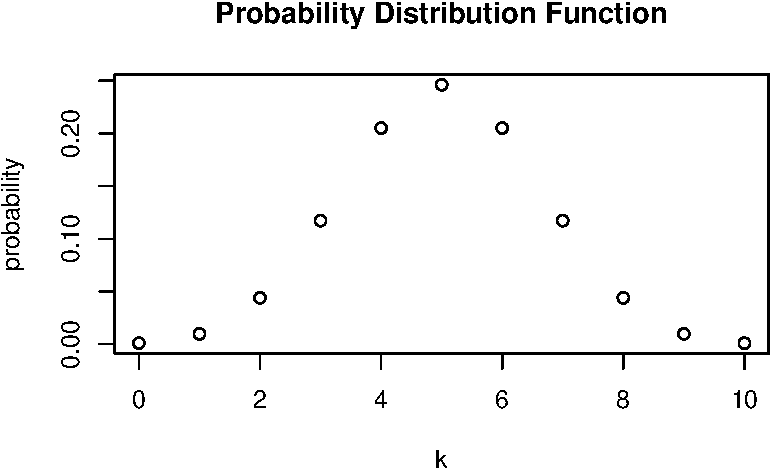
\includegraphics{URFITE_files/figure-latex/unnamed-chunk-19-1} \end{center}

We observe that, according to the estimated model equation, a
payment-to-income ratio of \(1\) is associated with an expected
probability of mortgage application denial of roughly \(50\%\). The
model indicates that there is a positive relation between the
payment-to-income ratio and the probability of a denied mortgage
application so individuals with a high ratio of loan payments to income
are more likely to be rejected.

We may use \texttt{coeftest()} to obtain robust standard errors for both
coefficient estimates.

\begin{Shaded}
\begin{Highlighting}[]
\CommentTok{# model coefficient summary}
\KeywordTok{coeftest}\NormalTok{(denymod1, }\DataTypeTok{vcov. =} \KeywordTok{vcovHC}\NormalTok{(denymod1, }\DataTypeTok{type =} \StringTok{"HC1"}\NormalTok{))}
\end{Highlighting}
\end{Shaded}

\begin{verbatim}
## 
## t test of coefficients:
## 
##              Estimate Std. Error t value  Pr(>|t|)    
## (Intercept) -0.079910   0.031967 -2.4998   0.01249 *  
## pirat        0.603535   0.098483  6.1283 1.036e-09 ***
## ---
## Signif. codes:  0 '***' 0.001 '**' 0.01 '*' 0.05 '.' 0.1 ' ' 1
\end{verbatim}

The estimated regression line is
\[\widehat{deny} = -\underset{(0.032)}{0.080} + \underset{(0.098)}{0.604} P/I \ ratio.\]
The true coefficient on \(P/I \ ratio\) is statistically different from
\(0\) at the \(1\%\) level. Its estimate can be interpreted as follows:
a \(1\%\) increase in \(P/I \ ratio\) leads to an increase in the
probability of a loan denial by
\(0.604 * 0.01 = 0.00604 \approx 0.6\%\).

Following the book we augment the simple model \eqref{eq:denymod1} by an
additional regressor \(black\) which equals \(1\) if the applicant is an
African American and equals \(0\) if the applicant is white. Such a
specification is the baseline for investigation of the question whether
there is racial discrimination in the mortgage market: if being black
has a significant (positive) influence on the probability of a loan
denial when we control for factors that allow for an objective
assessment of an applicants credit worthiness, this is an indicator for
discrimination.

\begin{Shaded}
\begin{Highlighting}[]
\CommentTok{# rename variable `afam`}
\KeywordTok{colnames}\NormalTok{(HMDA)[}\KeywordTok{colnames}\NormalTok{(HMDA) }\OperatorTok{==}\StringTok{ "afam"}\NormalTok{] <-}\StringTok{ "black"}

\CommentTok{# estimate the model}
\NormalTok{denymod2 <-}\StringTok{ }\KeywordTok{lm}\NormalTok{(deny }\OperatorTok{~}\StringTok{ }\NormalTok{pirat }\OperatorTok{+}\StringTok{ }\NormalTok{black, }\DataTypeTok{data =}\NormalTok{ HMDA)}
\KeywordTok{coeftest}\NormalTok{(denymod2, }\DataTypeTok{vcov. =} \KeywordTok{vcovHC}\NormalTok{(denymod2))}
\end{Highlighting}
\end{Shaded}

\begin{verbatim}
## 
## t test of coefficients:
## 
##              Estimate Std. Error t value  Pr(>|t|)    
## (Intercept) -0.090514   0.033430 -2.7076  0.006826 ** 
## pirat        0.559195   0.103671  5.3939 7.575e-08 ***
## blackyes     0.177428   0.025055  7.0815 1.871e-12 ***
## ---
## Signif. codes:  0 '***' 0.001 '**' 0.01 '*' 0.05 '.' 0.1 ' ' 1
\end{verbatim}

So the estimated regression function is

\begin{align}
  \widehat{deny} =& \, -\underset{(0.029)}{0.091} + \underset{(0.089)}{0.559} P/I \ ratio + \underset{(0.025)}{0.177} black. \label{eq:denymod2}
\end{align}

The coefficient on \(black\) is positive and significantly different
from zero at the \(0.01\%\) level. The interpretation is that, holding
constant the \(P/I \ ratio\), being black increases the probability of a
mortgage application denial by about \(17.7\%\). This suggests racial
discrimination. However, this result might be distorted by omitted
variable bias so this could be a premature conclusion.

\section{Probit and Logit Regression}\label{probit-and-logit-regression}

The linear probability model has a major flaw: it assumes the
conditional probability function to be linear. This does not restrict
the probability of observing \(Y=1\) conditional on some regressor to
lie between \(0\) and \(1\). We can easily see this in our reproduction
of Figure 11.1 of the book: for \(P/I \ ratio \geq 1.75\), model
\eqref{eq:denymod1} predicts the probability of a mortgage application
denial to be bigger than \(1\). For applications with \(P/I \ ratio\)
close to \(0\), the predicted probability of denial is even negative so
the model has no meaningful interpretation here.

This circumstance demands for an approach that use a \emph{nonlinear}
function to model the conditional probability function of a binary
dependent variable. Commonly used methods are Probit and Logit
regression.

\subsection*{Probit Regression}\label{probit-regression}
\addcontentsline{toc}{subsection}{Probit Regression}

In Probit regression, the cumulative standard normal distribution
function \(\Phi\) is used to model the regression function when the
dependent variable is binary, that is we assume

\begin{align}
  E(Y\vert X) = P(Y=1\vert X) = \Phi(\beta_0 + \beta_1 X). \label{eq:probitmodel}
\end{align}

\(\beta_0 + \beta_1 X\) in \eqref{eq:probitmodel} plays the role of a
quantile \(z\). Remember that
\[\Phi(z) = P(Z \leq z) \ , \ Z \sim \mathcal{N}(0,1).\] such that the
Probit coefficient \(\beta_1\) in \eqref{eq:probitmodel} is the change in
\(z\) associated with a one unit change in \(X\). Note that, although
the effect on \(z\) of a change in \(X\) is linear, the link between
\(z\) and the dependent variable \(Y\) is nonlinear since \(\Phi\) is a
nonlinear function of \(X\).

Since in Probit models the dependent variable is a nonlinear function of
the regressors, the coefficient on \(X\) has no simple interpretation.
According to Key Concept 8.1, the expected change in the probability
that \(Y=1\) due to a change in \(P/I \ ratio\) can be computed in the
following manner:

\begin{enumerate}
\def\labelenumi{\arabic{enumi}.}
\tightlist
\item
  Compute the predicted probability that \(Y=1\) for the original value
  of \(X\).
\item
  Compute the predicted probability that \(Y=1\) for \(X + \Delta X\).
\item
  Compute the difference between both predicted probabilities.
\end{enumerate}

Of course we can generalize \eqref{eq:probitmodel} to Probit regression
with multiple regressors to mitigate the risk of facing omitted variable
bias. The core knowledge on Probit regression is summarized in Key
Concept 11.2.

\begin{keyconcepts}[Probit Model, Predicted Probabilities and Estimated Effects]{11.2}
Assume that $Y$ is a binary variable. The model

$$ Y= \beta_0 + \beta_1 + X_1 + \beta_2 X_2 + \dots + \beta_k X_k + u $$
with
$$P(Y = 1 \vert X_1, X_2, \dots ,X_k) = \Phi(\beta_0 + \beta_1 + X_1 + \beta_2 X_2 + \dots + \beta_k X_k)$$
is the population Probit model with multiple regressors where $X_1, X_2, \dots, X_k$ are regressors and $\Phi$ is the cumulative standard normal distribution function.\newline

The predicted probability that $Y=1$ given $X_1, X_2, \dots, X_k$ can be calculated in two steps:\newline

\begin{enumerate}
\item Compute $z = \beta_0 + \beta_1 X_1 + \beta_2 X_2 + \dots + \beta_k X_k$
\item Look up $\Phi(z)$ using a normal distribution table or by calling \texttt{pnorm()}.
\end{enumerate}\vspace{0.5cm}

$\beta_j$ is the effect on $z$ of a one unit change in regressor $X_j$, holding constant all other $k-1$ regressors.\newline

The effect on the predicted probability of a change in a regressor can be computed as shown in Key Concept 8.1.\newline

In \texttt{R}, Probit models can be estimated using the function \texttt{glm()} from the package \texttt{stats}. Using the argument \texttt{family} we specify that we want to use a Probit link function.
\end{keyconcepts}

We now estimate a simple Probit model of the probability of a mortgage
denial.

\begin{Shaded}
\begin{Highlighting}[]
\CommentTok{# estimate the simple probit model}
\NormalTok{denyprobit <-}\StringTok{ }\KeywordTok{glm}\NormalTok{(deny }\OperatorTok{~}\StringTok{ }\NormalTok{pirat, }
                \DataTypeTok{family =} \KeywordTok{binomial}\NormalTok{(}\DataTypeTok{link =} \StringTok{"probit"}\NormalTok{), }
                \DataTypeTok{data =}\NormalTok{ HMDA)}

\KeywordTok{coeftest}\NormalTok{(denyprobit, }\DataTypeTok{vcov. =} \KeywordTok{vcovHC}\NormalTok{(denyprobit, }\DataTypeTok{type =} \StringTok{"HC1"}\NormalTok{))}
\end{Highlighting}
\end{Shaded}

\begin{verbatim}
## 
## z test of coefficients:
## 
##             Estimate Std. Error  z value  Pr(>|z|)    
## (Intercept) -2.19415    0.18901 -11.6087 < 2.2e-16 ***
## pirat        2.96787    0.53698   5.5269 3.259e-08 ***
## ---
## Signif. codes:  0 '***' 0.001 '**' 0.01 '*' 0.05 '.' 0.1 ' ' 1
\end{verbatim}

The estimated model equation is

\begin{align}
  \widehat{P(deny\vert P/I \ ratio}) = \Phi(-\underset{(0.19)}{2.19} + \underset{(0.54)}{2.97} P/I \ ratio). \label{eq:denyprobit}
\end{align}

Just as in the linear probability model we find that the relation
between the probability of denial and the payments-to-income ratio is
positive and that the corresponding coefficient is highly significant.

The following code chunk reproduces Figure 11.2 of the book.

\begin{Shaded}
\begin{Highlighting}[]
\CommentTok{# plot data}
\KeywordTok{plot}\NormalTok{(}\DataTypeTok{x =}\NormalTok{ HMDA}\OperatorTok{$}\NormalTok{pirat, }
\NormalTok{     HMDA}\OperatorTok{$}\NormalTok{deny,}
     \DataTypeTok{main =} \StringTok{"Probit Model of the Probability of Denial, Given P/I Ratio"}\NormalTok{,}
     \DataTypeTok{xlab =} \StringTok{"P/I ratio"}\NormalTok{,}
     \DataTypeTok{ylab =} \StringTok{"Deny"}\NormalTok{,}
     \DataTypeTok{pch =} \DecValTok{20}\NormalTok{,}
     \DataTypeTok{ylim =} \KeywordTok{c}\NormalTok{(}\OperatorTok{-}\FloatTok{0.4}\NormalTok{, }\FloatTok{1.4}\NormalTok{),}
     \DataTypeTok{cex.main =} \FloatTok{0.85}
\NormalTok{)}

\CommentTok{# add horizontal dashed lines and text}
\KeywordTok{abline}\NormalTok{(}\DataTypeTok{h =} \DecValTok{1}\NormalTok{, }\DataTypeTok{lty =} \DecValTok{2}\NormalTok{, }\DataTypeTok{col =} \StringTok{"darkred"}\NormalTok{)}
\KeywordTok{abline}\NormalTok{(}\DataTypeTok{h =} \DecValTok{0}\NormalTok{, }\DataTypeTok{lty =} \DecValTok{2}\NormalTok{, }\DataTypeTok{col =} \StringTok{"darkred"}\NormalTok{)}
\KeywordTok{text}\NormalTok{(}\FloatTok{2.5}\NormalTok{, }\FloatTok{0.9}\NormalTok{, }\DataTypeTok{cex =} \FloatTok{0.8}\NormalTok{, }\StringTok{"Mortgage denied"}\NormalTok{)}
\KeywordTok{text}\NormalTok{(}\FloatTok{2.5}\NormalTok{, }\OperatorTok{-}\FloatTok{0.1}\NormalTok{, }\DataTypeTok{cex=} \FloatTok{0.8}\NormalTok{, }\StringTok{"Mortgage approved"}\NormalTok{)}

\CommentTok{# add estimated regression line}
\NormalTok{x <-}\StringTok{ }\KeywordTok{seq}\NormalTok{(}\DecValTok{0}\NormalTok{, }\DecValTok{3}\NormalTok{, }\FloatTok{0.01}\NormalTok{)}
\NormalTok{y <-}\StringTok{ }\KeywordTok{predict}\NormalTok{(denyprobit, }\KeywordTok{list}\NormalTok{(}\DataTypeTok{pirat =}\NormalTok{ x), }\DataTypeTok{type =} \StringTok{"response"}\NormalTok{)}

\KeywordTok{lines}\NormalTok{(x, y, }\DataTypeTok{lwd =} \FloatTok{1.5}\NormalTok{, }\DataTypeTok{col =} \StringTok{"steelblue"}\NormalTok{)}
\end{Highlighting}
\end{Shaded}

\begin{center}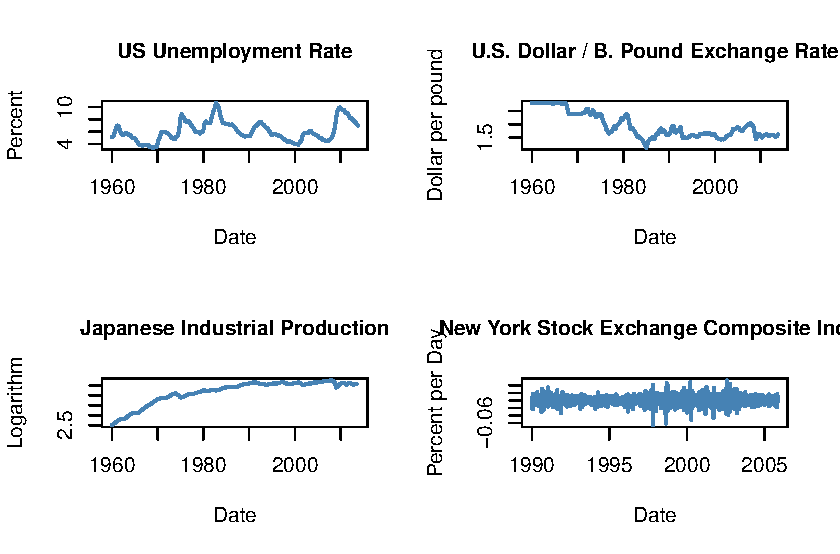
\includegraphics{URFITE_files/figure-latex/unnamed-chunk-25-1} \end{center}

Notice that the estimated regression function has a stretched
``S''-shape which is typical for the CDF of a of continuous random
variable with symmetric PDF like that of a normally distributed random
variable. The function is clearly nonlinear and flattens out for large
and small values of \(P/I \ ratio\). More importantly, the functional
form ensures that the predicted conditional probabilities of a denial
lie between \(0\) and \(1\).

We may use \texttt{predict()} to compute the predicted change in the
denial probability when \(P/I \ ratio\) is increased from \(0.3\) to
\(0.4\).

\begin{Shaded}
\begin{Highlighting}[]
\CommentTok{# 1. compute predictions for P/I ratio = 0.3, 0.4}
\NormalTok{predictions <-}\StringTok{ }\KeywordTok{predict}\NormalTok{(denyprobit, }
                       \DataTypeTok{newdata =} \KeywordTok{data.frame}\NormalTok{(}\StringTok{"pirat"}\NormalTok{ =}\StringTok{ }\KeywordTok{c}\NormalTok{(}\FloatTok{0.3}\NormalTok{, }\FloatTok{0.4}\NormalTok{)),}
                       \DataTypeTok{type =} \StringTok{"response"}
\NormalTok{                       )}

\CommentTok{# 2. Compute difference in probabilities}
\KeywordTok{diff}\NormalTok{(predictions)}
\end{Highlighting}
\end{Shaded}

\begin{verbatim}
##          2 
## 0.06081433
\end{verbatim}

We find that an increase in the payment-to-income ratio from \(0.3\) to
\(0.4\) is predicted to increase the probability of denial by
approximately \(6.2\%\).

We continue by using an augmented Probit model to estimate the effect of
race on the probability of a mortgage application denial.

\begin{Shaded}
\begin{Highlighting}[]
\NormalTok{denyprobit2 <-}\StringTok{ }\KeywordTok{glm}\NormalTok{(deny }\OperatorTok{~}\StringTok{ }\NormalTok{pirat }\OperatorTok{+}\StringTok{ }\NormalTok{black, }
                \DataTypeTok{family =} \KeywordTok{binomial}\NormalTok{(}\DataTypeTok{link =} \StringTok{"probit"}\NormalTok{), }
                \DataTypeTok{data =}\NormalTok{ HMDA)}

\KeywordTok{coeftest}\NormalTok{(denyprobit2, }\DataTypeTok{vcov. =} \KeywordTok{vcovHC}\NormalTok{(denyprobit2, }\DataTypeTok{type =} \StringTok{"HC1"}\NormalTok{))}
\end{Highlighting}
\end{Shaded}

\begin{verbatim}
## 
## z test of coefficients:
## 
##              Estimate Std. Error  z value  Pr(>|z|)    
## (Intercept) -2.258787   0.176608 -12.7898 < 2.2e-16 ***
## pirat        2.741779   0.497673   5.5092 3.605e-08 ***
## blackyes     0.708155   0.083091   8.5227 < 2.2e-16 ***
## ---
## Signif. codes:  0 '***' 0.001 '**' 0.01 '*' 0.05 '.' 0.1 ' ' 1
\end{verbatim}

The estimated model equation is

\begin{align}
  \widehat{P(deny\vert P/I \ ratio, black)} = \Phi (-\underset{(0.18)}{2.26} + \underset{(0.50)}{2.74} P/I \ ratio + \underset{(0.08)}{0.71} black). \label{eq:denyprobit2} 
\end{align}

While all coefficients are highly significant, both the estimated
coefficients on the payments-to-income ratio and the indicator for
African American descent are positive. Again, the coefficients are
difficult to interpret but they indicate that first, African Americans
have a higher probability of denial than white applicants do, holding
constant the payments-to-income ratio and second, applicants with a high
payments-to-income ratio face a higher risk of being rejected.

How big is the estimated difference in denial probabilities between two
hypothetical applicants with the same payments-to-income ratio? As
before, we may use \texttt{predict()} to compute this difference.

\begin{Shaded}
\begin{Highlighting}[]
\CommentTok{# 1. compute predictions for P/I ratio = 0.3,0.4}
\NormalTok{predictions <-}\StringTok{ }\KeywordTok{predict}\NormalTok{(denyprobit2, }
                       \DataTypeTok{newdata =} \KeywordTok{data.frame}\NormalTok{(}\StringTok{"black"}\NormalTok{ =}\StringTok{ }\KeywordTok{c}\NormalTok{(}\StringTok{"no"}\NormalTok{, }\StringTok{"yes"}\NormalTok{), }
                                            \StringTok{"pirat"}\NormalTok{ =}\StringTok{ }\KeywordTok{c}\NormalTok{(}\FloatTok{0.3}\NormalTok{, }\FloatTok{0.3}\NormalTok{)),}
                       \DataTypeTok{type =} \StringTok{"response"}
\NormalTok{                       )}

\CommentTok{# 2. Compute difference in probabilities}
\KeywordTok{diff}\NormalTok{(predictions)}
\end{Highlighting}
\end{Shaded}

\begin{verbatim}
##         2 
## 0.1578117
\end{verbatim}

In this case, the estimated difference in denial probabilities is about
\(15.8\%\).

\subsection*{Logit Regression}\label{logit-regression}
\addcontentsline{toc}{subsection}{Logit Regression}

Key Concept 11.3 summarizes the main differences between Logit and
Probit regression.

\begin{keyconcepts}[Logit Regression]{11.3}
The population Logit regression function is

\begin{align*}
  P(Y=1\vert X_1, X_2, \dots, X_k) =& \, F(\beta_0 + \beta_1 X_1 + \beta_2 X_2 + \dots + \beta_k X_k) \\
  =& \, \frac{1}{1+e^{-(\beta_0 + \beta_1 X_1 + \beta_2 X_2 + \dots + \beta_k X_k)}}.
\end{align*}

The idea is similar to Probit regression except that a different CDF is used: $$F(x) = \frac{1}{1+e^{-x}}$$ is the CDF of a standard logistically distributed random variable.
\end{keyconcepts}

As for Probit regression, there is no simple interpretation of the model
coefficients and it is best to consider predicted probabilities or
differences in predicted probabilities. Here again, \(t\)-statistics and
confidence intervals based on large sample normal approximations can be
computed as usual.

It is fairly easy to estimate a Logit regression model using \texttt{R}.

\begin{Shaded}
\begin{Highlighting}[]
\NormalTok{denylogit <-}\StringTok{ }\KeywordTok{glm}\NormalTok{(deny }\OperatorTok{~}\StringTok{ }\NormalTok{pirat, }
                \DataTypeTok{family =} \KeywordTok{binomial}\NormalTok{(}\DataTypeTok{link =} \StringTok{"logit"}\NormalTok{), }
                \DataTypeTok{data =}\NormalTok{ HMDA)}

\KeywordTok{coeftest}\NormalTok{(denylogit, }\DataTypeTok{vcov. =} \KeywordTok{vcovHC}\NormalTok{(denylogit, }\DataTypeTok{type =} \StringTok{"HC1"}\NormalTok{))}
\end{Highlighting}
\end{Shaded}

\begin{verbatim}
## 
## z test of coefficients:
## 
##             Estimate Std. Error  z value  Pr(>|z|)    
## (Intercept) -4.02843    0.35898 -11.2218 < 2.2e-16 ***
## pirat        5.88450    1.00015   5.8836 4.014e-09 ***
## ---
## Signif. codes:  0 '***' 0.001 '**' 0.01 '*' 0.05 '.' 0.1 ' ' 1
\end{verbatim}

The subsequent code chunk reproduces Figure 11.3 of the book.

\begin{Shaded}
\begin{Highlighting}[]
\CommentTok{# plot data}
\KeywordTok{plot}\NormalTok{(}\DataTypeTok{x =}\NormalTok{ HMDA}\OperatorTok{$}\NormalTok{pirat, }
\NormalTok{     HMDA}\OperatorTok{$}\NormalTok{deny,}
     \DataTypeTok{main =} \StringTok{"Probit and Logit Models Model of the Probability of Denial, Given P/I Ratio"}\NormalTok{,}
     \DataTypeTok{xlab =} \StringTok{"P/I ratio"}\NormalTok{,}
     \DataTypeTok{ylab =} \StringTok{"Deny"}\NormalTok{,}
     \DataTypeTok{pch =} \DecValTok{20}\NormalTok{,}
     \DataTypeTok{ylim =} \KeywordTok{c}\NormalTok{(}\OperatorTok{-}\FloatTok{0.4}\NormalTok{, }\FloatTok{1.4}\NormalTok{),}
     \DataTypeTok{cex.main =} \FloatTok{0.9}
\NormalTok{)}

\CommentTok{# add horizontal dashed lines and text}
\KeywordTok{abline}\NormalTok{(}\DataTypeTok{h =} \DecValTok{1}\NormalTok{, }\DataTypeTok{lty =} \DecValTok{2}\NormalTok{, }\DataTypeTok{col =} \StringTok{"darkred"}\NormalTok{)}
\KeywordTok{abline}\NormalTok{(}\DataTypeTok{h =} \DecValTok{0}\NormalTok{, }\DataTypeTok{lty =} \DecValTok{2}\NormalTok{, }\DataTypeTok{col =} \StringTok{"darkred"}\NormalTok{)}
\KeywordTok{text}\NormalTok{(}\FloatTok{2.5}\NormalTok{, }\FloatTok{0.9}\NormalTok{, }\DataTypeTok{cex =} \FloatTok{0.8}\NormalTok{, }\StringTok{"Mortgage denied"}\NormalTok{)}
\KeywordTok{text}\NormalTok{(}\FloatTok{2.5}\NormalTok{, }\OperatorTok{-}\FloatTok{0.1}\NormalTok{, }\DataTypeTok{cex=} \FloatTok{0.8}\NormalTok{, }\StringTok{"Mortgage approved"}\NormalTok{)}

\CommentTok{# add estimated regression line of Probit and Logit models}
\NormalTok{x <-}\StringTok{ }\KeywordTok{seq}\NormalTok{(}\DecValTok{0}\NormalTok{, }\DecValTok{3}\NormalTok{, }\FloatTok{0.01}\NormalTok{)}
\NormalTok{y_probit <-}\StringTok{ }\KeywordTok{predict}\NormalTok{(denyprobit, }\KeywordTok{list}\NormalTok{(}\DataTypeTok{pirat =}\NormalTok{ x), }\DataTypeTok{type =} \StringTok{"response"}\NormalTok{)}
\NormalTok{y_logit <-}\StringTok{ }\KeywordTok{predict}\NormalTok{(denylogit, }\KeywordTok{list}\NormalTok{(}\DataTypeTok{pirat =}\NormalTok{ x), }\DataTypeTok{type =} \StringTok{"response"}\NormalTok{)}

\KeywordTok{lines}\NormalTok{(x, y_probit, }\DataTypeTok{lwd =} \FloatTok{1.5}\NormalTok{, }\DataTypeTok{col =} \StringTok{"steelblue"}\NormalTok{)}
\KeywordTok{lines}\NormalTok{(x, y_logit, }\DataTypeTok{lwd =} \FloatTok{1.5}\NormalTok{, }\DataTypeTok{col =} \StringTok{"black"}\NormalTok{, }\DataTypeTok{lty =} \DecValTok{2}\NormalTok{)}

\CommentTok{# add a legend}
\KeywordTok{legend}\NormalTok{(}\StringTok{"topleft"}\NormalTok{,}
       \DataTypeTok{horiz =} \OtherTok{TRUE}\NormalTok{,}
       \DataTypeTok{legend =} \KeywordTok{c}\NormalTok{(}\StringTok{"Probit"}\NormalTok{, }\StringTok{"Logit"}\NormalTok{),}
       \DataTypeTok{col =} \KeywordTok{c}\NormalTok{(}\StringTok{"steelblue"}\NormalTok{, }\StringTok{"black"}\NormalTok{), }
       \DataTypeTok{lty =} \KeywordTok{c}\NormalTok{(}\DecValTok{1}\NormalTok{, }\DecValTok{2}\NormalTok{))}
\end{Highlighting}
\end{Shaded}

\begin{center}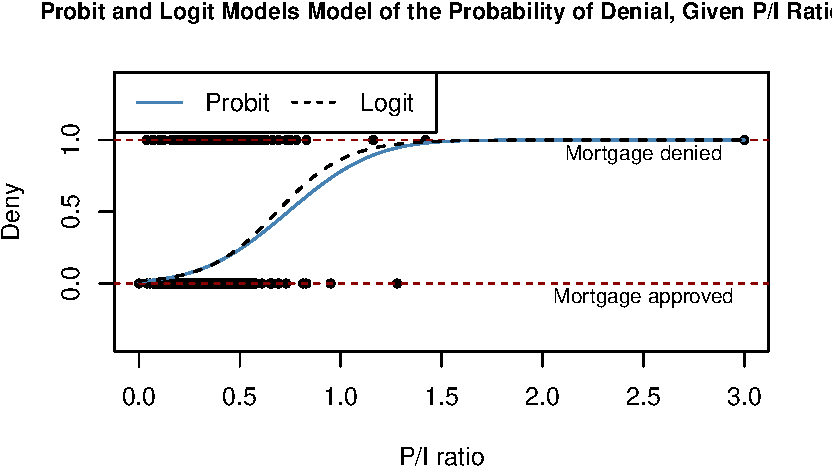
\includegraphics{URFITE_files/figure-latex/unnamed-chunk-32-1} \end{center}

Notice that both models produce very similar estimates of the
probability that a mortgage application will be denied depending on the
applicants payment-to-income ratio.

Following the book we expand the simple Logit model of mortgage denial
with the additional regressor \(black\).

\begin{Shaded}
\begin{Highlighting}[]
\CommentTok{# estimate Logit regression with multiple regressors}
\NormalTok{denylogit2 <-}\StringTok{ }\KeywordTok{glm}\NormalTok{(deny }\OperatorTok{~}\StringTok{ }\NormalTok{pirat }\OperatorTok{+}\StringTok{ }\NormalTok{black, }
                \DataTypeTok{family =} \KeywordTok{binomial}\NormalTok{(}\DataTypeTok{link =} \StringTok{"logit"}\NormalTok{), }
                \DataTypeTok{data =}\NormalTok{ HMDA)}

\KeywordTok{coeftest}\NormalTok{(denylogit2, }\DataTypeTok{vcov. =} \KeywordTok{vcovHC}\NormalTok{(denylogit2, }\DataTypeTok{type =} \StringTok{"HC1"}\NormalTok{))}
\end{Highlighting}
\end{Shaded}

\begin{verbatim}
## 
## z test of coefficients:
## 
##             Estimate Std. Error  z value  Pr(>|z|)    
## (Intercept) -4.12556    0.34597 -11.9245 < 2.2e-16 ***
## pirat        5.37036    0.96376   5.5723 2.514e-08 ***
## blackyes     1.27278    0.14616   8.7081 < 2.2e-16 ***
## ---
## Signif. codes:  0 '***' 0.001 '**' 0.01 '*' 0.05 '.' 0.1 ' ' 1
\end{verbatim}

We obtain

\begin{align}
  \widehat{P(deny=1 \vert P/I ratio, black)} = F(-\underset{(0.35)}{4.13} + \underset{(0.96)}{5.37} P/I \ ratio + \underset{(0.15)}{1.27} black). \label{eq:denylogit2}
\end{align}

As for the Probit model \eqref{eq:denyprobit2} all model coefficients are
highly significant and we obtain positive estimates for the coefficients
on \(P/I \ ratio\) and \(black\). For comparison purposes we compute the
predicted probability of denial for two hypothetical applicants that
differ in race and have a \(P/I \ ratio\) of \(0.3\).

\begin{Shaded}
\begin{Highlighting}[]
\CommentTok{# 1. compute predictions for P/I ratio = 0.3}
\NormalTok{predictions <-}\StringTok{ }\KeywordTok{predict}\NormalTok{(denylogit2, }
                       \DataTypeTok{newdata =} \KeywordTok{data.frame}\NormalTok{(}\StringTok{"black"}\NormalTok{ =}\StringTok{ }\KeywordTok{c}\NormalTok{(}\StringTok{"no"}\NormalTok{, }\StringTok{"yes"}\NormalTok{), }
                                            \StringTok{"pirat"}\NormalTok{ =}\StringTok{ }\KeywordTok{c}\NormalTok{(}\FloatTok{0.3}\NormalTok{, }\FloatTok{0.3}\NormalTok{)),}
                       \DataTypeTok{type =} \StringTok{"response"}
\NormalTok{                      )}

\NormalTok{predictions}
\end{Highlighting}
\end{Shaded}

\begin{verbatim}
##          1          2 
## 0.07485143 0.22414592
\end{verbatim}

\begin{Shaded}
\begin{Highlighting}[]
\CommentTok{# 2. Compute difference in probabilities}
\KeywordTok{diff}\NormalTok{(predictions)}
\end{Highlighting}
\end{Shaded}

\begin{verbatim}
##         2 
## 0.1492945
\end{verbatim}

We find that the white applicant faces a denial probability of only
\(7.5\%\), while the African American is rejected with a probability of
\(22.4\%\) with makes a difference of \(14.9\%\).

\subsubsection*{Comparison of the
Models}\label{comparison-of-the-models}
\addcontentsline{toc}{subsubsection}{Comparison of the Models}

The Probit model and the Logit model deliver only approximations to the
unknown population regression function \(E(Y\vert X)\). It is not
unambiguous to decide which model one should use in practice. The linear
probability model has the clear drawback of not being able to capture
the nonlinear nature of the population regression function and it
predicts probabilities to lie outside the interval \([0,1]\) for extreme
regressor values. Probit and Logit models are harder to interpret but
can capture the nonlinearities better than the linear approach: both
models produce predictions of probabilities that lie inside the interval
\([0,1]\). Predictions of Probit and Logit models are often close to
each other. The book suggests to use the method that is easiest to use
in the statistical software of choice. As we have seen, it is equally
easy to estimate Probit and Logit model using \texttt{R}. We can
therefore give no general recommendation which method to use.

\section{Estimation and Inference in the Logit and Probit
Models}\label{estimation-and-inference-in-the-logit-and-probit-models}

So far nothing has been said about \emph{how} Logit and Probit models
are estimated by statistical software. The reason why this is
interesting is that both models are \emph{nonlinear in the parameters}
and thus cannot be estimated using OLS. Instead one relies on a method
called \emph{maximum likelihood estimation} (MLE). Another approach is
estimation by \emph{nonlinear least squares} (NLS).

\subsubsection*{Nonlinear Least Squares}\label{nonlinear-least-squares}
\addcontentsline{toc}{subsubsection}{Nonlinear Least Squares}

Consider the multiple regression Probit model

\begin{align}
  E(Y_i\vert X_{1i}, \dots, X_{ki}) = P(Y_i=1\vert X_{1i}, \dots, X_{ki}) = \Phi(\beta_0 + \beta_1 X_{1i} + \dots + \beta_k X_{ki}). \label{eq:multprobit}
\end{align}

Similarly to OLS, NLS estimates the parameters
\(\beta_0,\beta_1,\dots,\beta_k\) by minimizing the sum of squared
mistakes
\[\sum_{i=1}^n\left[ Y_i - \Phi(b_0 + b_1 X_{1i} + \dots + b_k X_{ki}) \right]^2.\]
NLS estimation is a consistent approach that produces estimates which
are normally distributed in large samples. In \texttt{R} there are
functions like \texttt{nls()} from package \texttt{stats} which provide
algorithms for solving nonlinear least squares problems. However, NLS is
inefficient, meaning that there are estimation techniques that have a
smaller variance which is why we will not dwell any further on this
topic.

\subsubsection*{Maximum Likelihood
Estimation}\label{maximum-likelihood-estimation}
\addcontentsline{toc}{subsubsection}{Maximum Likelihood Estimation}

In MLE we seek to estimate the unknown parameters choosing them such
that the likelihood of drawing the sample observed is maximized. This
probability is measured by means the likelihood function, the joint
probability distribution of the data treated as a function of the
unknown parameters. Put differently, the maximum likelihood estimates of
the unknown parameters are the values that result in a model which is
most likely to produce the data observed. It turns out that MLE is more
efficient than NLS.

As maximum likelihood estimates are normally distributed in large
samples, statistical inference for coefficients in nonlinear models like
Logit and Probit regression can be made using the same tools that are
used for linear regression models: we can compute \(t\)-statistics and
confidence intervals.

Many software packages use an MLE algorithm for estimation of nonlinear
models. The function \texttt{glm()} uses an algorithm named
\emph{iteratively reweighted least squares}.

\subsubsection*{Measures of Fit}\label{measures-of-fit}
\addcontentsline{toc}{subsubsection}{Measures of Fit}

It is important to be aware that the usual \(R^2\) and
\(\overline{R^2}\) are \emph{invalid} for nonlinear regression models.
The reason for this is simple: both measures are derived under the
assumption that the relation between the dependent and the explanatory
variable(s) is linear. This obviously does not hold for Probit and Logit
models thus \(R^2\) does not fall between \(0\) and \(1\) and there is
no meaningful interpretation. However, statistical software sometimes
reports these measures anyway.

There are many measures of fit for nonlinear regression models and there
is no consensus which one should be reported. The situation is even more
complicated because there is no measure of fit that is generally
applicable. For models with a binary response variable like \(deny\) one
could use the following rule: \newline If \(Y_i = 1\) and
\(\widehat{P(Y_i|X_{i1}, \dots, X_{ik})} > 0.5\) or if \(Y_i = 0\) and
\(\widehat{P(Y_i|X_{i1}, \dots, X_{ik})} < 0.5\), consider the \(Y_i\)
as correctly predicted. Otherwise \(Y_i\) is said to be incorrectly
predicted. The measure of fit is the share of correctly predicted
observations. The downside of such an approach is that it does not yield
information on the quality of the prediction.\footnote{Note that this is
  in contrast to the case of a numeric dependent variable where we use
  the squared errors for assessment of the quality of the prediction.}

An alternative to the latter are so called pseudo-\(R^2\) measures. In
order to measure the quality of the fit, these measures compare the
value of the maximized (log-)likelihood of the model with all regressors
(the \emph{full model}) to the likelihood of a model with no regressors
(\emph{null model}, regression on a constant).

For example, consider a Probit regression. The \(\text{pseudo-}R^2\) is
given by
\[\text{pseudo-}R^2 = 1 - \frac{\ln(f^{max}_{full})}{\ln(f^{max}_{null})}\]
where \(f^{max}_j \in [0,1]\) denotes the maximized likelihood for model
\(j\).

The reasoning behind this is that the maximized likelihood increases as
additional regressors are added to the model, similarly to the decrease
in \(SSR\) when regressors are added in a linear regression model. If
the full model has a similar maximized likelihood than the null model,
the full model does not really improve upon a model that uses only the
information in the dependent variable, so
\(\text{pseudo-}R^2 \approx 0\). If the full model fits the data very
good, the maximized likelihood should be close to \(1\) such that
\(\ln(f^{max}_{full}) \approx 0\) and \(\text{pseudo-}R^2 \approx 1\).
See Appendix 11.2 of the book for more on MLE and pseudo-\(R^2\)
measures.

\texttt{summary()} does not report \(\text{pseudo-}R^2\) for models
estimated by \texttt{glm()} but we can use the entries \emph{residual
deviance} (\texttt{deviance}) and \emph{null deviance}
(\texttt{null.deviance}) instead. These are computed as
\[\text{deviance} = -2 \times \left[\ln(f^{max}_{saturated}) - \ln(f^{max}_{full}) \right]\]
and

\[\text{null deviance} = -2 \times \left[\ln(f^{max}_{saturated}) - \ln(f^{max}_{null}) \right]\]
where \(f^{max}_{saturated}\) is the maximized likelihood for a model
which assumes that each observation has its own parameter (there are
\(n+1\) parameters to be estimated which leads to a perfect fit). For
models wit ah binary dependent variable, it holds that
\[\text{pseudo-}R^2 = 1 - \frac{\text{deviance}}{\text{null deviance}} = 1- \frac{\ln(f^{max}_{full})}{\ln(f^{max}_{null})}.\]

We now compute the \(\text{pseudo-}R^2\) for the augmented Probit model
of mortgage denial.

\begin{Shaded}
\begin{Highlighting}[]
\CommentTok{# compute pseudo-R2 for the probit model of mortgage denial}
\NormalTok{pseudoR2 <-}\StringTok{ }\DecValTok{1} \OperatorTok{-}\StringTok{ }\NormalTok{(denyprobit2}\OperatorTok{$}\NormalTok{deviance) }\OperatorTok{/}\StringTok{ }\NormalTok{(denyprobit2}\OperatorTok{$}\NormalTok{null.deviance)}
\NormalTok{pseudoR2}
\end{Highlighting}
\end{Shaded}

\begin{verbatim}
## [1] 0.08594259
\end{verbatim}

Another way to obtain the \(\text{pseudo-}R^2\) is to estimate the null
model using \texttt{glm()} and extract the maximized log-likelihoods for
both the null and the full model using the function \texttt{logLik()}.

\begin{Shaded}
\begin{Highlighting}[]
\CommentTok{# compute null model}
\NormalTok{denyprobit_null <-}\StringTok{ }\KeywordTok{glm}\NormalTok{(}\DataTypeTok{formula =}\NormalTok{ deny }\OperatorTok{~}\StringTok{ }\DecValTok{1}\NormalTok{, }
                       \DataTypeTok{family =} \KeywordTok{binomial}\NormalTok{(}\DataTypeTok{link =} \StringTok{"probit"}\NormalTok{), }
                       \DataTypeTok{data =}\NormalTok{ HMDA)}

\CommentTok{# compute the pseudo-R2 using `logLik`}
\DecValTok{1} \OperatorTok{-}\StringTok{ }\KeywordTok{logLik}\NormalTok{(denyprobit2)[}\DecValTok{1}\NormalTok{]}\OperatorTok{/}\KeywordTok{logLik}\NormalTok{(denyprobit_null)[}\DecValTok{1}\NormalTok{]}
\end{Highlighting}
\end{Shaded}

\begin{verbatim}
## [1] 0.08594259
\end{verbatim}

\section{Application to the Boston HMDA
Data}\label{application-to-the-boston-hmda-data}

Models \eqref{eq:denyprobit2} and \eqref{eq:denylogit2} indicate that denial
rates are higher for African American applicants holding constant
payment-to-income ratio. Both results could be wrong due to omitted
variable bias. In order to obtain a more trustworthy estimate of the
effect of being black on the probability of a mortgage application
denial we estimate a linear probability model as well as several Logit
and Probit models. We thereby control for financial variables and
additional applicant characteristics which are likely to influence the
probability of denial and differ between black and white applicants.

Sample averages as shown in Table 11.1 of the book can be easily
reproduced using the functions \texttt{mean()} (as usual for numeric
variables) and \texttt{prop.table()} (for factor variables).

\begin{Shaded}
\begin{Highlighting}[]
\CommentTok{# Mean P/I ratio}
\KeywordTok{mean}\NormalTok{(HMDA}\OperatorTok{$}\NormalTok{pirat)}
\end{Highlighting}
\end{Shaded}

\begin{verbatim}
## [1] 0.3308136
\end{verbatim}

\begin{Shaded}
\begin{Highlighting}[]
\CommentTok{# inhouse expense-to-total-income ratio}
\KeywordTok{mean}\NormalTok{(HMDA}\OperatorTok{$}\NormalTok{hirat)}
\end{Highlighting}
\end{Shaded}

\begin{verbatim}
## [1] 0.2553461
\end{verbatim}

\begin{Shaded}
\begin{Highlighting}[]
\CommentTok{# loan-to-value ratio}
\KeywordTok{mean}\NormalTok{(HMDA}\OperatorTok{$}\NormalTok{lvrat)}
\end{Highlighting}
\end{Shaded}

\begin{verbatim}
## [1] 0.7377759
\end{verbatim}

\begin{Shaded}
\begin{Highlighting}[]
\CommentTok{# consumer credit score}
\KeywordTok{mean}\NormalTok{(}\KeywordTok{as.numeric}\NormalTok{(HMDA}\OperatorTok{$}\NormalTok{chist))}
\end{Highlighting}
\end{Shaded}

\begin{verbatim}
## [1] 2.116387
\end{verbatim}

\begin{Shaded}
\begin{Highlighting}[]
\CommentTok{# mortgage credit score}
\KeywordTok{mean}\NormalTok{(}\KeywordTok{as.numeric}\NormalTok{(HMDA}\OperatorTok{$}\NormalTok{mhist))}
\end{Highlighting}
\end{Shaded}

\begin{verbatim}
## [1] 1.721008
\end{verbatim}

\begin{Shaded}
\begin{Highlighting}[]
\CommentTok{# public bad credit record}
\KeywordTok{mean}\NormalTok{(}\KeywordTok{as.numeric}\NormalTok{(HMDA}\OperatorTok{$}\NormalTok{phist)}\OperatorTok{-}\DecValTok{1}\NormalTok{)}
\end{Highlighting}
\end{Shaded}

\begin{verbatim}
## [1] 0.07352941
\end{verbatim}

\begin{Shaded}
\begin{Highlighting}[]
\CommentTok{# denied mortgage insurance}
\KeywordTok{prop.table}\NormalTok{(}\KeywordTok{table}\NormalTok{(HMDA}\OperatorTok{$}\NormalTok{insurance))}
\end{Highlighting}
\end{Shaded}

\begin{verbatim}
## 
##         no        yes 
## 0.97983193 0.02016807
\end{verbatim}

\begin{Shaded}
\begin{Highlighting}[]
\CommentTok{# self-employed}
\KeywordTok{prop.table}\NormalTok{(}\KeywordTok{table}\NormalTok{(HMDA}\OperatorTok{$}\NormalTok{selfemp))}
\end{Highlighting}
\end{Shaded}

\begin{verbatim}
## 
##        no       yes 
## 0.8836134 0.1163866
\end{verbatim}

\begin{Shaded}
\begin{Highlighting}[]
\CommentTok{# single}
\KeywordTok{prop.table}\NormalTok{(}\KeywordTok{table}\NormalTok{(HMDA}\OperatorTok{$}\NormalTok{single))}
\end{Highlighting}
\end{Shaded}

\begin{verbatim}
## 
##        no       yes 
## 0.6067227 0.3932773
\end{verbatim}

\begin{Shaded}
\begin{Highlighting}[]
\CommentTok{# high school dimploma}
\KeywordTok{prop.table}\NormalTok{(}\KeywordTok{table}\NormalTok{(HMDA}\OperatorTok{$}\NormalTok{hschool))}
\end{Highlighting}
\end{Shaded}

\begin{verbatim}
## 
##         no        yes 
## 0.01638655 0.98361345
\end{verbatim}

\begin{Shaded}
\begin{Highlighting}[]
\CommentTok{# unemployment rate}
\KeywordTok{mean}\NormalTok{(HMDA}\OperatorTok{$}\NormalTok{unemp)}
\end{Highlighting}
\end{Shaded}

\begin{verbatim}
## [1] 3.774496
\end{verbatim}

\begin{Shaded}
\begin{Highlighting}[]
\CommentTok{# condominium}
\KeywordTok{prop.table}\NormalTok{(}\KeywordTok{table}\NormalTok{(HMDA}\OperatorTok{$}\NormalTok{condomin))}
\end{Highlighting}
\end{Shaded}

\begin{verbatim}
## 
##        no       yes 
## 0.7117647 0.2882353
\end{verbatim}

\begin{Shaded}
\begin{Highlighting}[]
\CommentTok{# black}
\KeywordTok{prop.table}\NormalTok{(}\KeywordTok{table}\NormalTok{(HMDA}\OperatorTok{$}\NormalTok{black))}
\end{Highlighting}
\end{Shaded}

\begin{verbatim}
## 
##       no      yes 
## 0.857563 0.142437
\end{verbatim}

\begin{Shaded}
\begin{Highlighting}[]
\CommentTok{# deny}
\KeywordTok{prop.table}\NormalTok{(}\KeywordTok{table}\NormalTok{(HMDA}\OperatorTok{$}\NormalTok{deny))}
\end{Highlighting}
\end{Shaded}

\begin{verbatim}
## 
##         0         1 
## 0.8802521 0.1197479
\end{verbatim}

See Chapter 11.4 of the book or use \texttt{R}'s help function for more
info on variables contained in the \texttt{HMDA} data set.

Before estimating the models we transform the loan-to-value ratio
(\texttt{lvrat}) into a factor variable, where

\begin{align*}
  lvrat = 
  \begin{cases}
    \text{low} & \text{if} \ \ lvrat < 0.8, \\
    \text{medium} & \text{if} \ \ 0.8 \leq lvrat \leq 0.95, \\
    \text{high} & \text{if} \ \ lvrat > 0.95
  \end{cases}
\end{align*}

and convert both credit scores to numeric variables.

\begin{Shaded}
\begin{Highlighting}[]
\CommentTok{# define low, medium and high loan-to-value ratio}
\NormalTok{HMDA}\OperatorTok{$}\NormalTok{lvrat <-}\StringTok{ }\KeywordTok{factor}\NormalTok{(}
  \KeywordTok{ifelse}\NormalTok{(HMDA}\OperatorTok{$}\NormalTok{lvrat }\OperatorTok{<}\StringTok{ }\FloatTok{0.8}\NormalTok{, }\StringTok{"low"}\NormalTok{,}
  \KeywordTok{ifelse}\NormalTok{(HMDA}\OperatorTok{$}\NormalTok{lvrat }\OperatorTok{>=}\StringTok{ }\FloatTok{0.8} \OperatorTok{&}\StringTok{ }\NormalTok{HMDA}\OperatorTok{$}\NormalTok{lvrat }\OperatorTok{<=}\StringTok{ }\FloatTok{0.95}\NormalTok{, }\StringTok{"medium"}\NormalTok{, }\StringTok{"high"}\NormalTok{)),}
  \DataTypeTok{levels =} \KeywordTok{c}\NormalTok{(}\StringTok{"low"}\NormalTok{, }\StringTok{"medium"}\NormalTok{, }\StringTok{"high"}\NormalTok{)}
\NormalTok{  )}

\CommentTok{# convert credit scores to numeric}
\NormalTok{HMDA}\OperatorTok{$}\NormalTok{mhist <-}\StringTok{ }\KeywordTok{as.numeric}\NormalTok{(HMDA}\OperatorTok{$}\NormalTok{mhist)}
\NormalTok{HMDA}\OperatorTok{$}\NormalTok{chist <-}\StringTok{ }\KeywordTok{as.numeric}\NormalTok{(HMDA}\OperatorTok{$}\NormalTok{chist)}
\end{Highlighting}
\end{Shaded}

In the next step we reproduce the estimation results presented in Table
11.2 of the book.

\begin{Shaded}
\begin{Highlighting}[]
\CommentTok{# estimate all 6 models for the denial probability}
\NormalTok{lpm_HMDA <-}\StringTok{ }\KeywordTok{lm}\NormalTok{(deny }\OperatorTok{~}\StringTok{ }\NormalTok{black }\OperatorTok{+}\StringTok{ }\NormalTok{pirat }\OperatorTok{+}\StringTok{ }\NormalTok{hirat }\OperatorTok{+}\StringTok{ }\NormalTok{lvrat }\OperatorTok{+}\StringTok{ }\NormalTok{chist }\OperatorTok{+}\StringTok{ }\NormalTok{mhist }\OperatorTok{+}\StringTok{ }\NormalTok{phist }
               \OperatorTok{+}\StringTok{ }\NormalTok{insurance }\OperatorTok{+}\StringTok{ }\NormalTok{selfemp, }\DataTypeTok{data =}\NormalTok{ HMDA)}

\NormalTok{logit_HMDA <-}\StringTok{ }\KeywordTok{glm}\NormalTok{(deny }\OperatorTok{~}\StringTok{ }\NormalTok{black }\OperatorTok{+}\StringTok{ }\NormalTok{pirat }\OperatorTok{+}\StringTok{ }\NormalTok{hirat }\OperatorTok{+}\StringTok{ }\NormalTok{lvrat }\OperatorTok{+}\StringTok{ }\NormalTok{chist }\OperatorTok{+}\StringTok{ }\NormalTok{mhist }\OperatorTok{+}\StringTok{ }\NormalTok{phist }
                  \OperatorTok{+}\StringTok{ }\NormalTok{insurance }\OperatorTok{+}\StringTok{ }\NormalTok{selfemp, }
                  \DataTypeTok{family =} \KeywordTok{binomial}\NormalTok{(}\DataTypeTok{link =} \StringTok{"logit"}\NormalTok{), }
                  \DataTypeTok{data =}\NormalTok{ HMDA)}

\NormalTok{probit_HMDA_}\DecValTok{1}\NormalTok{ <-}\StringTok{ }\KeywordTok{glm}\NormalTok{(deny }\OperatorTok{~}\StringTok{ }\NormalTok{black }\OperatorTok{+}\StringTok{ }\NormalTok{pirat }\OperatorTok{+}\StringTok{ }\NormalTok{hirat }\OperatorTok{+}\StringTok{ }\NormalTok{lvrat }\OperatorTok{+}\StringTok{ }\NormalTok{chist }\OperatorTok{+}\StringTok{ }\NormalTok{mhist }\OperatorTok{+}\StringTok{ }\NormalTok{phist }
                     \OperatorTok{+}\StringTok{ }\NormalTok{insurance }\OperatorTok{+}\StringTok{ }\NormalTok{selfemp, }
                     \DataTypeTok{family =} \KeywordTok{binomial}\NormalTok{(}\DataTypeTok{link =} \StringTok{"probit"}\NormalTok{), }
                     \DataTypeTok{data =}\NormalTok{ HMDA)}

\NormalTok{probit_HMDA_}\DecValTok{2}\NormalTok{ <-}\StringTok{ }\KeywordTok{glm}\NormalTok{(deny }\OperatorTok{~}\StringTok{ }\NormalTok{black }\OperatorTok{+}\StringTok{ }\NormalTok{pirat }\OperatorTok{+}\StringTok{ }\NormalTok{hirat }\OperatorTok{+}\StringTok{ }\NormalTok{lvrat }\OperatorTok{+}\StringTok{ }\NormalTok{chist }\OperatorTok{+}\StringTok{ }\NormalTok{mhist }\OperatorTok{+}\StringTok{ }\NormalTok{phist }
                     \OperatorTok{+}\StringTok{ }\NormalTok{insurance }\OperatorTok{+}\StringTok{ }\NormalTok{selfemp }\OperatorTok{+}\StringTok{ }\NormalTok{single }\OperatorTok{+}\StringTok{ }\NormalTok{hschool }\OperatorTok{+}\StringTok{ }\NormalTok{unemp, }
                     \DataTypeTok{family =} \KeywordTok{binomial}\NormalTok{(}\DataTypeTok{link =} \StringTok{"probit"}\NormalTok{), }
                     \DataTypeTok{data =}\NormalTok{ HMDA)}

\NormalTok{probit_HMDA_}\DecValTok{3}\NormalTok{ <-}\StringTok{ }\KeywordTok{glm}\NormalTok{(deny }\OperatorTok{~}\StringTok{ }\NormalTok{black }\OperatorTok{+}\StringTok{ }\NormalTok{pirat }\OperatorTok{+}\StringTok{ }\NormalTok{hirat }\OperatorTok{+}\StringTok{ }\NormalTok{lvrat }\OperatorTok{+}\StringTok{ }\NormalTok{chist }\OperatorTok{+}\StringTok{ }\NormalTok{mhist }
                     \OperatorTok{+}\StringTok{ }\NormalTok{phist }\OperatorTok{+}\StringTok{ }\NormalTok{insurance }\OperatorTok{+}\StringTok{ }\NormalTok{selfemp }\OperatorTok{+}\StringTok{ }\NormalTok{single }\OperatorTok{+}\StringTok{ }\NormalTok{hschool }\OperatorTok{+}\StringTok{ }\NormalTok{unemp }\OperatorTok{+}\StringTok{ }\NormalTok{condomin }
                     \OperatorTok{+}\StringTok{ }\KeywordTok{I}\NormalTok{(mhist}\OperatorTok{==}\DecValTok{3}\NormalTok{) }\OperatorTok{+}\StringTok{ }\KeywordTok{I}\NormalTok{(mhist}\OperatorTok{==}\DecValTok{4}\NormalTok{) }\OperatorTok{+}\StringTok{ }\KeywordTok{I}\NormalTok{(chist}\OperatorTok{==}\DecValTok{3}\NormalTok{) }\OperatorTok{+}\StringTok{ }\KeywordTok{I}\NormalTok{(chist}\OperatorTok{==}\DecValTok{4}\NormalTok{) }\OperatorTok{+}\StringTok{ }\KeywordTok{I}\NormalTok{(chist}\OperatorTok{==}\DecValTok{5}\NormalTok{) }
                     \OperatorTok{+}\StringTok{ }\KeywordTok{I}\NormalTok{(chist}\OperatorTok{==}\DecValTok{6}\NormalTok{), }
                     \DataTypeTok{family =} \KeywordTok{binomial}\NormalTok{(}\DataTypeTok{link =} \StringTok{"probit"}\NormalTok{), }
                     \DataTypeTok{data =}\NormalTok{ HMDA)}

\NormalTok{probit_HMDA_}\DecValTok{4}\NormalTok{ <-}\StringTok{ }\KeywordTok{glm}\NormalTok{(deny }\OperatorTok{~}\StringTok{ }\NormalTok{black }\OperatorTok{*}\StringTok{ }\NormalTok{(pirat }\OperatorTok{+}\StringTok{ }\NormalTok{hirat) }\OperatorTok{+}\StringTok{ }\NormalTok{lvrat }\OperatorTok{+}\StringTok{ }\NormalTok{chist }\OperatorTok{+}\StringTok{ }\NormalTok{mhist }\OperatorTok{+}\StringTok{ }\NormalTok{phist }
                     \OperatorTok{+}\StringTok{ }\NormalTok{insurance }\OperatorTok{+}\StringTok{ }\NormalTok{selfemp }\OperatorTok{+}\StringTok{ }\NormalTok{single }\OperatorTok{+}\StringTok{ }\NormalTok{hschool }\OperatorTok{+}\StringTok{ }\NormalTok{unemp, }
                     \DataTypeTok{family =} \KeywordTok{binomial}\NormalTok{(}\DataTypeTok{link =} \StringTok{"probit"}\NormalTok{), }
                     \DataTypeTok{data =}\NormalTok{ HMDA)}
\end{Highlighting}
\end{Shaded}

Just as in previous chapters, we use the package \texttt{sandwich} for
computation of heteroskedasticity-robust standard errors of the
coefficient estimators in all models and store these in an object of the
type \texttt{list} which is then used as the argument \texttt{se} in
\texttt{stargazer()}.

\begin{Shaded}
\begin{Highlighting}[]
\KeywordTok{library}\NormalTok{(stargazer)}

\NormalTok{rob_se <-}\StringTok{ }\KeywordTok{list}\NormalTok{(}
  \KeywordTok{sqrt}\NormalTok{(}\KeywordTok{diag}\NormalTok{(}\KeywordTok{vcovHC}\NormalTok{(lpm_HMDA, }\DataTypeTok{type =} \StringTok{"HC1"}\NormalTok{))),}
  \KeywordTok{sqrt}\NormalTok{(}\KeywordTok{diag}\NormalTok{(}\KeywordTok{vcovHC}\NormalTok{(logit_HMDA, }\DataTypeTok{type =} \StringTok{"HC1"}\NormalTok{))),}
  \KeywordTok{sqrt}\NormalTok{(}\KeywordTok{diag}\NormalTok{(}\KeywordTok{vcovHC}\NormalTok{(probit_HMDA_}\DecValTok{1}\NormalTok{, }\DataTypeTok{type =} \StringTok{"HC1"}\NormalTok{))),}
  \KeywordTok{sqrt}\NormalTok{(}\KeywordTok{diag}\NormalTok{(}\KeywordTok{vcovHC}\NormalTok{(probit_HMDA_}\DecValTok{2}\NormalTok{, }\DataTypeTok{type =} \StringTok{"HC1"}\NormalTok{))),}
  \KeywordTok{sqrt}\NormalTok{(}\KeywordTok{diag}\NormalTok{(}\KeywordTok{vcovHC}\NormalTok{(probit_HMDA_}\DecValTok{3}\NormalTok{, }\DataTypeTok{type =} \StringTok{"HC1"}\NormalTok{))),}
  \KeywordTok{sqrt}\NormalTok{(}\KeywordTok{diag}\NormalTok{(}\KeywordTok{vcovHC}\NormalTok{(probit_HMDA_}\DecValTok{4}\NormalTok{, }\DataTypeTok{type =} \StringTok{"HC1"}\NormalTok{)))}
\NormalTok{)}

\KeywordTok{stargazer}\NormalTok{(lpm_HMDA, logit_HMDA, probit_HMDA_}\DecValTok{1}\NormalTok{, probit_HMDA_}\DecValTok{2}\NormalTok{, probit_HMDA_}\DecValTok{3}\NormalTok{, probit_HMDA_}\DecValTok{4}\NormalTok{,  }
          \DataTypeTok{digits =} \DecValTok{3}\NormalTok{,}
          \DataTypeTok{type =} \StringTok{"latex"}\NormalTok{, }
          \DataTypeTok{header =} \OtherTok{FALSE}\NormalTok{,}
          \DataTypeTok{se =}\NormalTok{ rob_se,}
          \DataTypeTok{model.numbers =} \OtherTok{FALSE}\NormalTok{,}
          \DataTypeTok{column.labels =} \KeywordTok{c}\NormalTok{(}\StringTok{"(1)"}\NormalTok{, }\StringTok{"(2)"}\NormalTok{, }\StringTok{"(3)"}\NormalTok{, }\StringTok{"(4)"}\NormalTok{, }\StringTok{"(5)"}\NormalTok{, }\StringTok{"(6)"}\NormalTok{)}
\NormalTok{          )}
\end{Highlighting}
\end{Shaded}

\begin{sidewaystable}[!htbp] \centering 
  \caption{\label{tab:hmdad} HMDA Data: LPM, Probit and Logit Models} 
  \label{} 
\begin{tabular}{@{\extracolsep{-5pt}}lcccccc} 
\\[-1.8ex]\hline 
\hline \\[-1.8ex] 
 & \multicolumn{6}{c}{\textit{Dependent variable:}} \\ 
\cline{2-7} 
\\[-1.8ex] & \multicolumn{6}{c}{deny} \\ 
\\[-1.8ex] & \textit{OLS} & \textit{logistic} & \multicolumn{4}{c}{\textit{probit}} \\ 
 & (1) & (2) & (3) & (4) & (5) & (6) \\ 
\hline \\[-1.8ex] 
 blackyes & 0.084$^{***}$ (0.023) & 0.688$^{***}$ (0.183) & 0.389$^{***}$ (0.099) & 0.371$^{***}$ (0.100) & 0.363$^{***}$ (0.101) & 0.246 (0.479) \\ 
  pirat & 0.449$^{***}$ (0.114) & 4.764$^{***}$ (1.332) & 2.442$^{***}$ (0.673) & 2.464$^{***}$ (0.654) & 2.622$^{***}$ (0.665) & 2.572$^{***}$ (0.728) \\ 
  hirat & $-$0.048 (0.110) & $-$0.109 (1.298) & $-$0.185 (0.689) & $-$0.302 (0.689) & $-$0.502 (0.715) & $-$0.538 (0.755) \\ 
  lvratmedium & 0.031$^{**}$ (0.013) & 0.464$^{***}$ (0.160) & 0.214$^{***}$ (0.082) & 0.216$^{***}$ (0.082) & 0.215$^{**}$ (0.084) & 0.216$^{***}$ (0.083) \\ 
  lvrathigh & 0.189$^{***}$ (0.050) & 1.495$^{***}$ (0.325) & 0.791$^{***}$ (0.183) & 0.795$^{***}$ (0.184) & 0.836$^{***}$ (0.185) & 0.788$^{***}$ (0.185) \\ 
  chist & 0.031$^{***}$ (0.005) & 0.290$^{***}$ (0.039) & 0.155$^{***}$ (0.021) & 0.158$^{***}$ (0.021) & 0.344$^{***}$ (0.108) & 0.158$^{***}$ (0.021) \\ 
  mhist & 0.021$^{*}$ (0.011) & 0.279$^{**}$ (0.138) & 0.148$^{**}$ (0.073) & 0.110 (0.076) & 0.162 (0.104) & 0.111 (0.077) \\ 
  phistyes & 0.197$^{***}$ (0.035) & 1.226$^{***}$ (0.203) & 0.697$^{***}$ (0.114) & 0.702$^{***}$ (0.115) & 0.717$^{***}$ (0.116) & 0.705$^{***}$ (0.115) \\ 
  insuranceyes & 0.702$^{***}$ (0.045) & 4.548$^{***}$ (0.576) & 2.557$^{***}$ (0.305) & 2.585$^{***}$ (0.299) & 2.589$^{***}$ (0.306) & 2.590$^{***}$ (0.299) \\ 
  selfempyes & 0.060$^{***}$ (0.021) & 0.666$^{***}$ (0.214) & 0.359$^{***}$ (0.113) & 0.346$^{***}$ (0.116) & 0.342$^{***}$ (0.116) & 0.348$^{***}$ (0.116) \\ 
  singleyes &  &  &  & 0.229$^{***}$ (0.080) & 0.230$^{***}$ (0.086) & 0.226$^{***}$ (0.081) \\ 
  hschoolyes &  &  &  & $-$0.613$^{***}$ (0.229) & $-$0.604$^{**}$ (0.237) & $-$0.620$^{***}$ (0.229) \\ 
  unemp &  &  &  & 0.030$^{*}$ (0.018) & 0.028 (0.018) & 0.030 (0.018) \\ 
  condominyes &  &  &  &  & $-$0.055 (0.096) &  \\ 
  I(mhist == 3) &  &  &  &  & $-$0.107 (0.301) &  \\ 
  I(mhist == 4) &  &  &  &  & $-$0.383 (0.427) &  \\ 
  I(chist == 3) &  &  &  &  & $-$0.226 (0.248) &  \\ 
  I(chist == 4) &  &  &  &  & $-$0.251 (0.338) &  \\ 
  I(chist == 5) &  &  &  &  & $-$0.789$^{*}$ (0.412) &  \\ 
  I(chist == 6) &  &  &  &  & $-$0.905$^{*}$ (0.515) &  \\ 
  blackyes:pirat &  &  &  &  &  & $-$0.579 (1.550) \\ 
  blackyes:hirat &  &  &  &  &  & 1.232 (1.709) \\ 
  Constant & $-$0.183$^{***}$ (0.028) & $-$5.707$^{***}$ (0.484) & $-$3.041$^{***}$ (0.250) & $-$2.575$^{***}$ (0.350) & $-$2.896$^{***}$ (0.404) & $-$2.543$^{***}$ (0.370) \\ 
 \hline \\[-1.8ex] 
Observations & 2,380 & 2,380 & 2,380 & 2,380 & 2,380 & 2,380 \\ 
R$^{2}$ & 0.266 &  &  &  &  &  \\ 
Adjusted R$^{2}$ & 0.263 &  &  &  &  &  \\ 
Log Likelihood &  & $-$635.637 & $-$636.847 & $-$628.614 & $-$625.064 & $-$628.332 \\ 
Akaike Inf. Crit. &  & 1,293.273 & 1,295.694 & 1,285.227 & 1,292.129 & 1,288.664 \\ 
Residual Std. Error & 0.279 (df = 2369) &  &  &  &  &  \\ 
F Statistic & 85.974$^{***}$ (df = 10; 2369) &  &  &  &  &  \\ 
\hline 
\hline \\[-1.8ex] 
\textit{Note:}  & \multicolumn{6}{r}{$^{*}$p$<$0.1; $^{**}$p$<$0.05; $^{***}$p$<$0.01} \\ 
\end{tabular} 
\end{sidewaystable}

In Table \ref{tab:hmdad}, models (1), (2) and (3) are base
specifications that include several financial control variables. They
differ only in the way they model the denial probability. Model (1) is a
linear probability model, model (2) is a Logit regression and model (3)
uses the Probit approach.

Since model (1) is a linear model, the coefficients have direct
interpretation. For example, an increase in the consumer credit score by
\(1\) unit is estimated to increase the probability of a loan denial by
about \(0.031\) percentage points. We also find that having a high
loan-to-value ratio is predicted not to be conductive for credit
approval: the coefficient for a loan-to-value ratio higher than \(0.95\)
is \(0.189\) so clients with this property are estimated to face an
almost \(19\%\) larger risk of denial than those with a low
loan-to-value ratio, ceteris paribus. For the linear probability model,
the coefficient on the race dummy is estimated to be \(0.084\) which
indicates the denial probability for African Americans is \(8.4\%\)
larger than for white applicants with the same characteristics except
for race. Apart from housing expense-to-income ratio and the mortgage
credit score, all coefficients are significant.

Models (2) and (3) provide similar evidence that there is racial
discrimination in the U.S. mortgage market. All coefficients except for
housing expense-to-income ratio (which is not significantly different
from zero) are significant at the \(1\%\) level. As discussed above, the
nonlinearity makes the interpretation of the coefficient estimates more
difficult than for model (1). In order to make a statement about the
effect of being black, we need to compute the estimated denial
probability for two individuals that differ only in race. For the
comparison we consider two individuals that share mean values for all
numeric regressors. For all qualitative variables we assign the property
that is the most representative for the data at hand. As an example,
consider self-employment: we have seen that about \(88\%\) of all
individuals in the sample are not self-employed such that we set
\texttt{selfemp = no}. Using this approach, the estimate for the effect
on the denial probability of being African American obtained using the
Logit model (2) is about \(4\%\). The next code chunk shows how to apply
this approach for models (1) to (7) using \texttt{R}.

\begin{Shaded}
\begin{Highlighting}[]
\CommentTok{# regressor values for average person, black = "yes"}
\NormalTok{new <-}\StringTok{ }\KeywordTok{data.frame}\NormalTok{(}
  \StringTok{"pirat"}\NormalTok{ =}\StringTok{ }\KeywordTok{mean}\NormalTok{(HMDA}\OperatorTok{$}\NormalTok{pirat),}
  \StringTok{"hirat"}\NormalTok{ =}\StringTok{ }\KeywordTok{mean}\NormalTok{(HMDA}\OperatorTok{$}\NormalTok{hirat),}
  \StringTok{"lvrat"}\NormalTok{ =}\StringTok{ "low"}\NormalTok{,}
  \StringTok{"chist"}\NormalTok{ =}\StringTok{ }\KeywordTok{mean}\NormalTok{(HMDA}\OperatorTok{$}\NormalTok{chist),}
  \StringTok{"mhist"}\NormalTok{ =}\StringTok{ }\KeywordTok{mean}\NormalTok{(HMDA}\OperatorTok{$}\NormalTok{mhist),}
  \StringTok{"phist"}\NormalTok{ =}\StringTok{ "no"}\NormalTok{,}
  \StringTok{"insurance"}\NormalTok{ =}\StringTok{ "no"}\NormalTok{,}
  \StringTok{"selfemp"}\NormalTok{ =}\StringTok{ "no"}\NormalTok{,}
  \StringTok{"black"}\NormalTok{ =}\StringTok{ }\KeywordTok{c}\NormalTok{(}\StringTok{"no"}\NormalTok{, }\StringTok{"yes"}\NormalTok{),}
  \StringTok{"single"}\NormalTok{ =}\StringTok{ "no"}\NormalTok{,}
  \StringTok{"hschool"}\NormalTok{ =}\StringTok{ "yes"}\NormalTok{,}
  \StringTok{"unemp"}\NormalTok{ =}\StringTok{ }\KeywordTok{mean}\NormalTok{(HMDA}\OperatorTok{$}\NormalTok{unemp),}
  \StringTok{"condomin"}\NormalTok{ =}\StringTok{ "no"}
\NormalTok{)}

\CommentTok{# differnce predicted by the LPM}
\NormalTok{predictions <-}\StringTok{ }\KeywordTok{predict}\NormalTok{(lpm_HMDA, }\DataTypeTok{newdata =}\NormalTok{ new)}
\KeywordTok{diff}\NormalTok{(predictions)}
\end{Highlighting}
\end{Shaded}

\begin{verbatim}
##          2 
## 0.08369674
\end{verbatim}

\begin{Shaded}
\begin{Highlighting}[]
\CommentTok{# differnce predicted by the logit model}
\NormalTok{predictions <-}\StringTok{ }\KeywordTok{predict}\NormalTok{(logit_HMDA, }\DataTypeTok{newdata =}\NormalTok{ new, }\DataTypeTok{type =} \StringTok{"response"}\NormalTok{)}
\KeywordTok{diff}\NormalTok{(predictions)}
\end{Highlighting}
\end{Shaded}

\begin{verbatim}
##          2 
## 0.04042135
\end{verbatim}

\begin{Shaded}
\begin{Highlighting}[]
\CommentTok{# difference predicted by probit model (3)}
\NormalTok{predictions <-}\StringTok{ }\KeywordTok{predict}\NormalTok{(probit_HMDA_}\DecValTok{1}\NormalTok{, }\DataTypeTok{newdata =}\NormalTok{ new, }\DataTypeTok{type =} \StringTok{"response"}\NormalTok{)}
\KeywordTok{diff}\NormalTok{(predictions)}
\end{Highlighting}
\end{Shaded}

\begin{verbatim}
##          2 
## 0.05049716
\end{verbatim}

\begin{Shaded}
\begin{Highlighting}[]
\CommentTok{# difference predicted by probit model (4)}
\NormalTok{predictions <-}\StringTok{ }\KeywordTok{predict}\NormalTok{(probit_HMDA_}\DecValTok{2}\NormalTok{, }\DataTypeTok{newdata =}\NormalTok{ new, }\DataTypeTok{type =} \StringTok{"response"}\NormalTok{)}
\KeywordTok{diff}\NormalTok{(predictions)}
\end{Highlighting}
\end{Shaded}

\begin{verbatim}
##          2 
## 0.03978918
\end{verbatim}

\begin{Shaded}
\begin{Highlighting}[]
\CommentTok{# difference predicted by probit model (5)}
\NormalTok{predictions <-}\StringTok{ }\KeywordTok{predict}\NormalTok{(probit_HMDA_}\DecValTok{3}\NormalTok{, }\DataTypeTok{newdata =}\NormalTok{ new, }\DataTypeTok{type =} \StringTok{"response"}\NormalTok{)}
\KeywordTok{diff}\NormalTok{(predictions)}
\end{Highlighting}
\end{Shaded}

\begin{verbatim}
##          2 
## 0.04972468
\end{verbatim}

\begin{Shaded}
\begin{Highlighting}[]
\CommentTok{# difference predicted by probit model (6)}
\NormalTok{predictions <-}\StringTok{ }\KeywordTok{predict}\NormalTok{(probit_HMDA_}\DecValTok{4}\NormalTok{, }\DataTypeTok{newdata =}\NormalTok{ new, }\DataTypeTok{type =} \StringTok{"response"}\NormalTok{)}
\KeywordTok{diff}\NormalTok{(predictions)}
\end{Highlighting}
\end{Shaded}

\begin{verbatim}
##          2 
## 0.03955893
\end{verbatim}

The estimates of the impact on the denial probability of being black are
similar for models (2) and (3). In particular, it is interesting that
the magnitude of the estimated effects is much smaller than for Probit
and Logit models that do not control for financial characteristics (see
section 11.2). This indicates that these simple models produce biased
estimates due to omitted variables.

Regressions (4) to (6) use regression specifications that include
different sets of applicant characteristics and credit rating indicator
variables as well as interactions. However, most of the corresponding
coefficients are not significant and the estimates of the coefficient on
\texttt{black} obtained for these models as well as the estimated
difference in denial probabilities do not deviate much from those
obtained for the similar specifications (2) and (3).

An interesting question related to racial discrimination can be
investigated using the Probit model (6) where the interactions
\texttt{blackyes:pirat} and \texttt{blackyes:hirat} are added to the the
specification of model (4). If the coefficient on
\texttt{blackyes:pirat} was different from zero, the effect of the
payment-to-income ratio on the denial probability would be different for
black and white applicants. Similarly, a non-zero coefficient on
\texttt{blackyes:hirat} would indicate that loan officers weight the
risk of bankrupt associated with a high loan-to-value ratio differently
for black and white mortgage applicants. We can test whether these
coefficients are jointly significant at the \(5\%\) level using an
\(F\)-Test.

\begin{Shaded}
\begin{Highlighting}[]
\KeywordTok{linearHypothesis}\NormalTok{(probit_HMDA_}\DecValTok{4}\NormalTok{,}
                 \DataTypeTok{test =} \StringTok{"F"}\NormalTok{,}
                 \KeywordTok{c}\NormalTok{(}\StringTok{"blackyes:pirat=0"}\NormalTok{, }\StringTok{"blackyes:hirat=0"}\NormalTok{),}
                 \DataTypeTok{vcov =} \KeywordTok{vcovHC}\NormalTok{(probit_HMDA_}\DecValTok{4}\NormalTok{, }\DataTypeTok{type =} \StringTok{"HC1"}\NormalTok{))}
\end{Highlighting}
\end{Shaded}

\begin{verbatim}
## Linear hypothesis test
## 
## Hypothesis:
## blackyes:pirat = 0
## blackyes:hirat = 0
## 
## Model 1: restricted model
## Model 2: deny ~ black * (pirat + hirat) + lvrat + chist + mhist + phist + 
##     insurance + selfemp + single + hschool + unemp
## 
## Note: Coefficient covariance matrix supplied.
## 
##   Res.Df Df      F Pr(>F)
## 1   2366                 
## 2   2364  2 0.2616 0.7698
\end{verbatim}

Since \(p\text{-value} \approx 0.77\) for this test, the null cannot be
rejected. Nonetheless, we cannot reject the hypothesis that there is no
racial discrimination at all since the corresponding \(F\)-test has a
\(p\text{-value}\) of about \(0.002\).

\begin{Shaded}
\begin{Highlighting}[]
\KeywordTok{linearHypothesis}\NormalTok{(probit_HMDA_}\DecValTok{4}\NormalTok{,}
                 \DataTypeTok{test =} \StringTok{"F"}\NormalTok{,}
                 \KeywordTok{c}\NormalTok{(}\StringTok{"blackyes=0"}\NormalTok{, }\StringTok{"blackyes:pirat=0"}\NormalTok{, }\StringTok{"blackyes:hirat=0"}\NormalTok{),}
                 \DataTypeTok{vcov =} \KeywordTok{vcovHC}\NormalTok{(probit_HMDA_}\DecValTok{4}\NormalTok{, }\DataTypeTok{type =} \StringTok{"HC1"}\NormalTok{))}
\end{Highlighting}
\end{Shaded}

\begin{verbatim}
## Linear hypothesis test
## 
## Hypothesis:
## blackyes = 0
## blackyes:pirat = 0
## blackyes:hirat = 0
## 
## Model 1: restricted model
## Model 2: deny ~ black * (pirat + hirat) + lvrat + chist + mhist + phist + 
##     insurance + selfemp + single + hschool + unemp
## 
## Note: Coefficient covariance matrix supplied.
## 
##   Res.Df Df      F   Pr(>F)   
## 1   2367                      
## 2   2364  3 4.8886 0.002168 **
## ---
## Signif. codes:  0 '***' 0.001 '**' 0.01 '*' 0.05 '.' 0.1 ' ' 1
\end{verbatim}

\subsubsection*{Summary}\label{summary}
\addcontentsline{toc}{subsubsection}{Summary}

Models (1) to (6) provide evidence that there is an effect of being
African American on the probability of a mortgage application denial: in
all specifications, the effect is estimated to be positive (ranging from
\(4\%\) to \(5\%\) for the fictive individuals considered) and is
significantly different from zero at the \(1\%\) level. While the linear
probability model seems to overestimate this effect slightly, it still
can be used as an approximation to an intrinsic nonlinear relationship.

See Chapters 11.4 and 11.5 of the book for a discussion of external and
internal validity of this study and some concluding remarks on
regression models where the dependent variable is binary.

\bibliography{book.bib,packages.bib}


\end{document}
